\documentclass[acmsmall]{acmart}

\usepackage{amsmath,amsfonts}
\usepackage{algorithmic}
\usepackage{graphicx}
\usepackage{textcomp}
\usepackage{xcolor}
\usepackage{caption}
\usepackage{comment}
\usepackage{xspace}
\usepackage{booktabs}
\usepackage{listings}
\usepackage{float}
\usepackage{longtable}
\usepackage{array}
\usepackage{url}
\usepackage[lined, algonl, ruled, boxed,vlined,linesnumbered]{algorithm2e} 
%\usepackage{algpseudocode}
\usepackage{ragged2e}

%%
%% \BibTeX command to typeset BibTeX logo in the docs
\AtBeginDocument{%
  \providecommand\BibTeX{{%
    Bib\TeX}}}

%% Rights management information.  This information is sent to you
%% when you complete the rights form.  These commands have SAMPLE
%% values in them; it is your responsibility as an author to replace
%% the commands and values with those provided to you when you
%% complete the rights form.

%% These commands are for a PROCEEDINGS abstract or paper.
% \acmConference[FSE '25]{the ACM on Software Engineering}{June 23--27, 2025}{Trondheim, Norway}
%%
%%  Uncomment \acmBooktitle if the title of the proceedings is different
%%  from ``Proceedings of ...''!
%%
%%\acmBooktitle{Woodstock '18: ACM Symposium on Neural Gaze Detection,
%%  June 03--05, 2018, Woodstock, NY}
% \acmISBN{978-1-4503-XXXX-X/18/06}    

\lstset{
  basicstyle=\footnotesize, % Use footnotesize for better readability
  xleftmargin=3ex,
  columns=fullflexible,
  numbers=left,
  frame=tb,
  escapeinside={(*}{*)},
  breaklines=true,
  numbersep=2pt,
  abovecaptionskip=5pt % Adjust the space above the caption as needed
}

\newcolumntype{L}[1]{>{\raggedright\let\newline\\\arraybackslash\hspace{0pt}}m{#1}}
\newcolumntype{C}[1]{>{\centering\let\newline\\\arraybackslash\hspace{0pt}}m{#1}}
\newcolumntype{R}[1]{>{\raggedleft\let\newline\\\arraybackslash\hspace{0pt}}m{#1}}

\newcommand{\tool}{\textsc{MeCheck}\xspace}
\newcommand{\todo} [1]{\textcolor{blue}{{\sf TODO}: #1}}
\newcommand{\codefont}[1]{\footnotesize{\texttt{#1}}\normalsize}
% \newcommand{\totalRule}{9\xspace}
\newcommand{\totalRule}{15\xspace}
\newcommand{\totalFunc}{41\xspace}
\newcommand{\precision}{100\%\xspace}
\newcommand{\recall}{96\%\xspace}
\newcommand{\fscore}{98\%\xspace}
\newcommand{\totalProject}{831\xspace}

% \newcommand{\totalReportedInReal}{155\xspace}
\newcommand{\totalReportedInReal}{{152}\xspace}
% \newcommand{\totalInteresting}{120\xspace}
\newcommand{\totalInteresting}{{117}\xspace}
\newcommand{\totalInterestingEAs}{21\xspace}
% \newcommand{\totalRealBugs}{52\xspace}
\newcommand{\totalRealBugs}{{49}\xspace}
\newcommand{\totalFalsePositives}{35\xspace}
\newcommand{\totalInjectedProject}{45\xspace}
\newcommand{\totalInjection}{45\xspace}
\newcommand{\totalProjectIncluded}{115\xspace}
\newcommand{\totalRealProject}{70\xspace}
\newcommand{\red} [1]{\textcolor{red}{#1}}

%%% The following is specific to FSE '25 and the paper
%%% 'Detecting Metadata-Related Bugs in Enterprise Applications'
%%% by Md Mahir Asef Kabir, Xiaoyin Wang, and Na Meng.
%%%
\setcopyright{cc}
\setcctype{by}
\acmDOI{10.1145/3715772}
\acmYear{2025}
\acmJournal{PACMSE}
\acmVolume{2}
\acmNumber{FSE}
\acmArticle{FSE053}
\acmMonth{7}
\received{2024-09-05}
\received[accepted]{2025-01-14}

%%
%% end of the preamble, start of the body of the document source.
\begin{document}

%%
%% The "title" command has an optional parameter,
%% allowing the author to define a "short title" to be used in page headers.
\title{Detecting Metadata-Related Bugs in Enterprise Applications}
\subtitle{This paper will appear in the Proceedings of the 2025 ACM International Conference on the Foundations of Software Engineering (FSE 2025).}


\author{Md Mahir Asef Kabir}
\email{mdmahirasefk@vt.edu}
\orcid{0000-0001-6227-1816}
\affiliation{%
  \institution{Virginia Tech}
  \city{Blacksburg}
  \state{Virginia}
  \country{USA}
}

\author{Xiaoyin Wang}
\orcid{0000-0002-9079-5534}
\affiliation{%
  \institution{The University of Texas at San Antonio}
  \city{San Antonio}
  \state{Texas}
  \country{USA}
}
\email{xiaoyin.wang@utsa.edu}

\author{Na Meng}
\orcid{0000-0002-0230-5524}
\affiliation{%
  \institution{Virginia Tech}
  \city{Blacksburg}
  \state{Virginia}
  \country{USA}
}
\email{nm8247@vt.edu}

\begin{abstract}  
Test time scaling is currently one of the most active research areas that shows promise after training time scaling has reached its limits.
Deep-thinking (DT) models are a class of recurrent models that can perform easy-to-hard generalization by assigning more compute to harder test samples.
However, due to their inability to determine the complexity of a test sample, DT models have to use a large amount of computation for both easy and hard test samples.
Excessive test time computation is wasteful and can cause the ``overthinking'' problem where more test time computation leads to worse results.
In this paper, we introduce a test time training method for determining the optimal amount of computation needed for each sample during test time.
We also propose Conv-LiGRU, a novel recurrent architecture for efficient and robust visual reasoning. 
Extensive experiments demonstrate that Conv-LiGRU is more stable than DT, effectively mitigates the ``overthinking'' phenomenon, and achieves superior accuracy.
\end{abstract}  


\begin{CCSXML}
<ccs2012>
   <concept>
       <concept_id>10011007.10011006.10011060.10011690</concept_id>
       <concept_desc>Software and its engineering~Specification languages</concept_desc>
       <concept_significance>500</concept_significance>
       </concept>
   <concept>
       <concept_id>10011007.10011006.10011041.10010943</concept_id>
       <concept_desc>Software and its engineering~Interpreters</concept_desc>
       <concept_significance>500</concept_significance>
       </concept>
   <concept>
       <concept_id>10011007.10011006.10011041.10011688</concept_id>
       <concept_desc>Software and its engineering~Parsers</concept_desc>
       <concept_significance>100</concept_significance>
       </concept>
   <concept>
       <concept_id>10011007.10011006.10011073</concept_id>
       <concept_desc>Software and its engineering~Software maintenance tools</concept_desc>
       <concept_significance>300</concept_significance>
       </concept>
 </ccs2012>
\end{CCSXML}

\ccsdesc[500]{Software and its engineering~Specification languages}
\ccsdesc[500]{Software and its engineering~Interpreters}
\ccsdesc[300]{Software and its engineering~Software maintenance tools}
\ccsdesc[100]{Software and its engineering~Parsers}



\keywords{Domain-specific language, metadata, XML, annotation, consistency}


\maketitle

\section{Introduction}
\label{sec:introduction}
The business processes of organizations are experiencing ever-increasing complexity due to the large amount of data, high number of users, and high-tech devices involved \cite{martin2021pmopportunitieschallenges, beerepoot2023biggestbpmproblems}. This complexity may cause business processes to deviate from normal control flow due to unforeseen and disruptive anomalies \cite{adams2023proceddsriftdetection}. These control-flow anomalies manifest as unknown, skipped, and wrongly-ordered activities in the traces of event logs monitored from the execution of business processes \cite{ko2023adsystematicreview}. For the sake of clarity, let us consider an illustrative example of such anomalies. Figure \ref{FP_ANOMALIES} shows a so-called event log footprint, which captures the control flow relations of four activities of a hypothetical event log. In particular, this footprint captures the control-flow relations between activities \texttt{a}, \texttt{b}, \texttt{c} and \texttt{d}. These are the causal ($\rightarrow$) relation, concurrent ($\parallel$) relation, and other ($\#$) relations such as exclusivity or non-local dependency \cite{aalst2022pmhandbook}. In addition, on the right are six traces, of which five exhibit skipped, wrongly-ordered and unknown control-flow anomalies. For example, $\langle$\texttt{a b d}$\rangle$ has a skipped activity, which is \texttt{c}. Because of this skipped activity, the control-flow relation \texttt{b}$\,\#\,$\texttt{d} is violated, since \texttt{d} directly follows \texttt{b} in the anomalous trace.
\begin{figure}[!t]
\centering
\includegraphics[width=0.9\columnwidth]{images/FP_ANOMALIES.png}
\caption{An example event log footprint with six traces, of which five exhibit control-flow anomalies.}
\label{FP_ANOMALIES}
\end{figure}

\subsection{Control-flow anomaly detection}
Control-flow anomaly detection techniques aim to characterize the normal control flow from event logs and verify whether these deviations occur in new event logs \cite{ko2023adsystematicreview}. To develop control-flow anomaly detection techniques, \revision{process mining} has seen widespread adoption owing to process discovery and \revision{conformance checking}. On the one hand, process discovery is a set of algorithms that encode control-flow relations as a set of model elements and constraints according to a given modeling formalism \cite{aalst2022pmhandbook}; hereafter, we refer to the Petri net, a widespread modeling formalism. On the other hand, \revision{conformance checking} is an explainable set of algorithms that allows linking any deviations with the reference Petri net and providing the fitness measure, namely a measure of how much the Petri net fits the new event log \cite{aalst2022pmhandbook}. Many control-flow anomaly detection techniques based on \revision{conformance checking} (hereafter, \revision{conformance checking}-based techniques) use the fitness measure to determine whether an event log is anomalous \cite{bezerra2009pmad, bezerra2013adlogspais, myers2018icsadpm, pecchia2020applicationfailuresanalysispm}. 

The scientific literature also includes many \revision{conformance checking}-independent techniques for control-flow anomaly detection that combine specific types of trace encodings with machine/deep learning \cite{ko2023adsystematicreview, tavares2023pmtraceencoding}. Whereas these techniques are very effective, their explainability is challenging due to both the type of trace encoding employed and the machine/deep learning model used \cite{rawal2022trustworthyaiadvances,li2023explainablead}. Hence, in the following, we focus on the shortcomings of \revision{conformance checking}-based techniques to investigate whether it is possible to support the development of competitive control-flow anomaly detection techniques while maintaining the explainable nature of \revision{conformance checking}.
\begin{figure}[!t]
\centering
\includegraphics[width=\columnwidth]{images/HIGH_LEVEL_VIEW.png}
\caption{A high-level view of the proposed framework for combining \revision{process mining}-based feature extraction with dimensionality reduction for control-flow anomaly detection.}
\label{HIGH_LEVEL_VIEW}
\end{figure}

\subsection{Shortcomings of \revision{conformance checking}-based techniques}
Unfortunately, the detection effectiveness of \revision{conformance checking}-based techniques is affected by noisy data and low-quality Petri nets, which may be due to human errors in the modeling process or representational bias of process discovery algorithms \cite{bezerra2013adlogspais, pecchia2020applicationfailuresanalysispm, aalst2016pm}. Specifically, on the one hand, noisy data may introduce infrequent and deceptive control-flow relations that may result in inconsistent fitness measures, whereas, on the other hand, checking event logs against a low-quality Petri net could lead to an unreliable distribution of fitness measures. Nonetheless, such Petri nets can still be used as references to obtain insightful information for \revision{process mining}-based feature extraction, supporting the development of competitive and explainable \revision{conformance checking}-based techniques for control-flow anomaly detection despite the problems above. For example, a few works outline that token-based \revision{conformance checking} can be used for \revision{process mining}-based feature extraction to build tabular data and develop effective \revision{conformance checking}-based techniques for control-flow anomaly detection \cite{singh2022lapmsh, debenedictis2023dtadiiot}. However, to the best of our knowledge, the scientific literature lacks a structured proposal for \revision{process mining}-based feature extraction using the state-of-the-art \revision{conformance checking} variant, namely alignment-based \revision{conformance checking}.

\subsection{Contributions}
We propose a novel \revision{process mining}-based feature extraction approach with alignment-based \revision{conformance checking}. This variant aligns the deviating control flow with a reference Petri net; the resulting alignment can be inspected to extract additional statistics such as the number of times a given activity caused mismatches \cite{aalst2022pmhandbook}. We integrate this approach into a flexible and explainable framework for developing techniques for control-flow anomaly detection. The framework combines \revision{process mining}-based feature extraction and dimensionality reduction to handle high-dimensional feature sets, achieve detection effectiveness, and support explainability. Notably, in addition to our proposed \revision{process mining}-based feature extraction approach, the framework allows employing other approaches, enabling a fair comparison of multiple \revision{conformance checking}-based and \revision{conformance checking}-independent techniques for control-flow anomaly detection. Figure \ref{HIGH_LEVEL_VIEW} shows a high-level view of the framework. Business processes are monitored, and event logs obtained from the database of information systems. Subsequently, \revision{process mining}-based feature extraction is applied to these event logs and tabular data input to dimensionality reduction to identify control-flow anomalies. We apply several \revision{conformance checking}-based and \revision{conformance checking}-independent framework techniques to publicly available datasets, simulated data of a case study from railways, and real-world data of a case study from healthcare. We show that the framework techniques implementing our approach outperform the baseline \revision{conformance checking}-based techniques while maintaining the explainable nature of \revision{conformance checking}.

In summary, the contributions of this paper are as follows.
\begin{itemize}
    \item{
        A novel \revision{process mining}-based feature extraction approach to support the development of competitive and explainable \revision{conformance checking}-based techniques for control-flow anomaly detection.
    }
    \item{
        A flexible and explainable framework for developing techniques for control-flow anomaly detection using \revision{process mining}-based feature extraction and dimensionality reduction.
    }
    \item{
        Application to synthetic and real-world datasets of several \revision{conformance checking}-based and \revision{conformance checking}-independent framework techniques, evaluating their detection effectiveness and explainability.
    }
\end{itemize}

The rest of the paper is organized as follows.
\begin{itemize}
    \item Section \ref{sec:related_work} reviews the existing techniques for control-flow anomaly detection, categorizing them into \revision{conformance checking}-based and \revision{conformance checking}-independent techniques.
    \item Section \ref{sec:abccfe} provides the preliminaries of \revision{process mining} to establish the notation used throughout the paper, and delves into the details of the proposed \revision{process mining}-based feature extraction approach with alignment-based \revision{conformance checking}.
    \item Section \ref{sec:framework} describes the framework for developing \revision{conformance checking}-based and \revision{conformance checking}-independent techniques for control-flow anomaly detection that combine \revision{process mining}-based feature extraction and dimensionality reduction.
    \item Section \ref{sec:evaluation} presents the experiments conducted with multiple framework and baseline techniques using data from publicly available datasets and case studies.
    \item Section \ref{sec:conclusions} draws the conclusions and presents future work.
\end{itemize}
% !TEX root = main.tex

\begin{figure}[t]
\vspace{-1.5cm}
\begin{minipage}{0.34\textwidth}
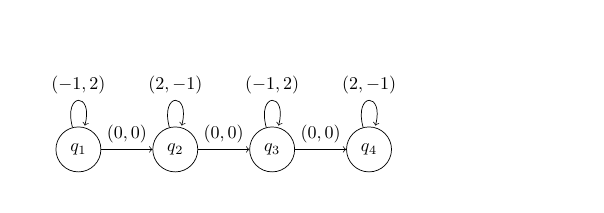
\begin{tikzpicture}[scale=0.25]
\usetikzlibrary{automata, positioning}
\scalebox{0.65}{
\node[state] (q1) {$q_1$};
\node[state, right=of q1] (q2) {$q_2$};
\node[state, right=of q2] (q3) {$q_3$};
\node[state, right=of q3] (q4) {$q_4$};

\path[->] (q1) edge [loop above] node[above] {$(-1,2)$} (q1) edge node[above] {$(0,0)$} (q2); 
\path[->] (q2) edge [loop above] node[above] {$(2,-1)$} (q2) edge node[above] {$(0,0)$} (q3);
\path[->] (q3) edge [loop above] node[above] {$(-1,2)$} (q3) edge node[above] {$(0,0)$} (q4);
\path[->] (q4) edge [loop above] node[above] {$(2,-1)$} (q4);
}
\end{tikzpicture}
\end{minipage}
\begin{minipage}{0.32\textwidth}
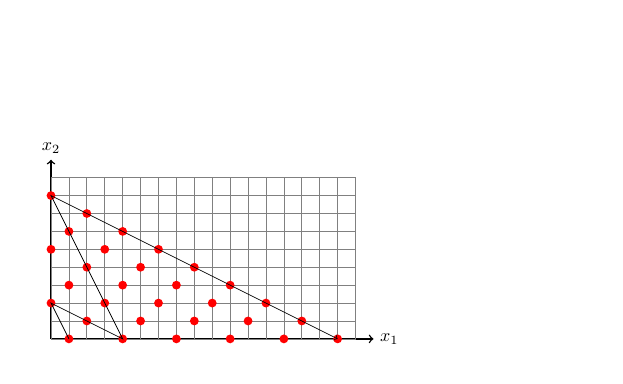
\begin{tikzpicture}[scale=0.35]
\scalebox{0.65}{
\draw[->, thick] (0, 0) -- (18, 0) node[right] {$x_1$};
\draw[->, thick] (0, 0) -- (0, 10) node[above] {$x_2$};

\draw[step=1, gray, thin] (0, 0) grid (17, 9);

\foreach \x in {1,4,7,10,13,16} \fill[red] (\x,0) circle (7pt);
\foreach \x in {2,5,8,11,14} \fill[red] (\x,1) circle (7pt);
\foreach \x in {0,3,6,9,12} \fill[red] (\x,2) circle (7pt);
\foreach \x in {1,4,7,10} \fill[red] (\x,3) circle (7pt);
\foreach \x in {2,5,8} \fill[red] (\x,4) circle (7pt);
\foreach \x in {0,3,6} \fill[red] (\x,5) circle (7pt);
\foreach \x in {1,4} \fill[red] (\x,6) circle (7pt);
\foreach \x in {2} \fill[red] (\x,7) circle (7pt);
\foreach \x in {0} \fill[red] (\x,8) circle (7pt);

\draw[->] (1,0) -- (0,2) -- (2,1) -- (4,0) -- (3,2) -- (2,4) -- (1,6) -- (0,8) -- (2,7) -- (4,6) -- (6,5) -- (8,4) -- (10,3) -- (12,2) -- (14,1) -- (16,0);
}
\end{tikzpicture}
\end{minipage}
\begin{minipage}{0.32\textwidth}
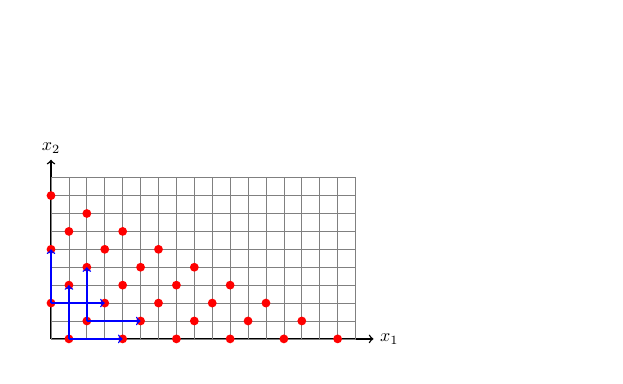
\begin{tikzpicture}[scale=0.35]
\scalebox{0.65}{
\draw[->, thick] (0, 0) -- (18, 0) node[right] {$x_1$};
\draw[->, thick] (0, 0) -- (0, 10) node[above] {$x_2$};

\draw[step=1, gray, thin] (0, 0) grid (17, 9);

\foreach \x in {1,4,7,10,13,16} \fill[red] (\x,0) circle (7pt);
\foreach \x in {2,5,8,11,14} \fill[red] (\x,1) circle (7pt);
\foreach \x in {0,3,6,9,12} \fill[red] (\x,2) circle (7pt);
\foreach \x in {1,4,7,10} \fill[red] (\x,3) circle (7pt);
\foreach \x in {2,5,8} \fill[red] (\x,4) circle (7pt);
\foreach \x in {0,3,6} \fill[red] (\x,5) circle (7pt);
\foreach \x in {1,4} \fill[red] (\x,6) circle (7pt);
\foreach \x in {2} \fill[red] (\x,7) circle (7pt);
\foreach \x in {0} \fill[red] (\x,8) circle (7pt);

\draw[->,blue,thick] (1,0) -- (4,0);
\draw[->,blue,thick] (1,0) -- (1,3);

\draw[->,blue,thick] (2,1) -- (5,1);
\draw[->,blue,thick] (2,1) -- (2,4);

\draw[->,blue,thick] (0,2) -- (3,2);
\draw[->,blue,thick] (0,2) -- (0,5);
}
\end{tikzpicture}
\end{minipage}
\caption{Left: 4-component \dvass $V_2$. 
Middle: the set $\reach_{q_4}(V_2, q_1(1,0))$ and a path $q_1(1,0) \tran q_4(16,0)$.
Right: bases 
%$A = \{(1,0),(2,1),(0,2)\}$ 
and periods 
%$P = \{(0,3),(3,0)\}$
 of an over-approximating semi-linear set $A+P^*$.}
\label{fig:zigzag}
\end{figure}

\begin{example}
For $k\geq 1$, let $V_k$ be a $(2k)$-component \dvass, where each component has just one state $q_i$
and one transition:
$(q_i, (-1,2), q_i)$ for odd $i$, and $(q_i, (2,-1), q_i)$ for even $i$.
Bridge transitions are $(q_i, (0,0), q_{i+1})$.
Figure~\ref{fig:zigzag} shows $V_2$ (left) and 
a path in $V_2$ from $s = q_1(1,0)$ to $t = q_4(16,0)$ together with 
the reachability set $\reach_{q_4}(V_2, s)$ (middle).
In general,
\begin{align} \label{eq:reachk}
X_k := \reach_{q_{2k}}(V_k, s) \ = \ \set{(x_1,x_2) \mid x_1+2x_2 \leq 4^k, \  x_1+2x_2 \equiv 1 \!\! \mod 3}.
\end{align}
Even if the size of the reachability set is 
exponential in $k$, for small $(x_1, x_2)$ it is periodic and the periods are small.
The set $X_k$ can be over-approximated by $A + P^*$ for $A = \set{(1,0),(2,1),(0,2)}$ and $P = \set{(0,3),(3,0)}$
(shown on the right of Figure~\ref{fig:zigzag}), namely for every $k\geq 1$ and $B\in\N$,
the set $X_k$ is \kanapka {$8$} {$B$}. 
For illustration, consider $Y := X_k \cap ((1,0) + P^*)$.
If $(1,0) + P^{\leq B} \subseteq X_k$ then $Y$ is a $B$-approximation
of $(1,0) + P^*$ with $\norm((1,0)), \norm(P) \leq 3 \leq 8$. 
Otherwise, there is some $(v_1, v_2) \in \big((1,0) + P^{\leq B}\big)\setminus X_k$, and
then $B$ is larger than $4^k$:
\[
%8B \geq 2(1 + 3B) \geq 2(v_1 + v_2) \geq v_1 + 2 v_2 > 
4^k < v_1 + 2 v_2 \leq 2(v_1 + v_2) \leq 2(1+3B) \leq 8B.
\]
Therefore by \eqref{eq:reachk}, each $(x_1,x_2) \in Y$ satisfies 
$\norm(x_1,x_2) = x_1 + x_2 \leq x_1 + 2x_2 \leq 4^k < 8B$, and thus
$Y$, seen as a union of singletons, is a union of 
linear sets with norm of base bounded by $8B$ and empty set of periods. 
In both cases, 
$Y$ is \kanapka {$8$} {$B$}. 
%The same intuition stays behind polynomial approximability of \dvass stated in Lemma~\ref{lem:2vass-sandwich}.
\end{example}
\section{Background}\label{sec:backgrnd}

\subsection{Cold Start Latency and Mitigation Techniques}

Traditional FaaS platforms mitigate cold starts through snapshotting, lightweight virtualization, and warm-state management. Snapshot-based methods like \textbf{REAP} and \textbf{Catalyzer} reduce initialization time by preloading or restoring container states but require significant memory and I/O resources, limiting scalability~\cite{dong_catalyzer_2020, ustiugov_benchmarking_2021}. Lightweight virtualization solutions, such as \textbf{Firecracker} microVMs, achieve fast startup times with strong isolation but depend on robust infrastructure, making them less adaptable to fluctuating workloads~\cite{agache_firecracker_2020}. Warm-state management techniques like \textbf{Faa\$T}~\cite{romero_faa_2021} and \textbf{Kraken}~\cite{vivek_kraken_2021} keep frequently invoked containers ready, balancing readiness and cost efficiency under predictable workloads but incurring overhead when demand is erratic~\cite{romero_faa_2021, vivek_kraken_2021}. While these methods perform well in resource-rich cloud environments, their resource intensity challenges applicability in edge settings.

\subsubsection{Edge FaaS Perspective}

In edge environments, cold start mitigation emphasizes lightweight designs, resource sharing, and hybrid task distribution. Lightweight execution environments like unikernels~\cite{edward_sock_2018} and \textbf{Firecracker}~\cite{agache_firecracker_2020}, as used by \textbf{TinyFaaS}~\cite{pfandzelter_tinyfaas_2020}, minimize resource usage and initialization delays but require careful orchestration to avoid resource contention. Function co-location, demonstrated by \textbf{Photons}~\cite{v_dukic_photons_2020}, reduces redundant initializations by sharing runtime resources among related functions, though this complicates isolation in multi-tenant setups~\cite{v_dukic_photons_2020}. Hybrid offloading frameworks like \textbf{GeoFaaS}~\cite{malekabbasi_geofaas_2024} balance edge-cloud workloads by offloading latency-tolerant tasks to the cloud and reserving edge resources for real-time operations, requiring reliable connectivity and efficient task management. These edge-specific strategies address cold starts effectively but introduce challenges in scalability and orchestration.

\subsection{Predictive Scaling and Caching Techniques}

Efficient resource allocation is vital for maintaining low latency and high availability in serverless platforms. Predictive scaling and caching techniques dynamically provision resources and reduce cold start latency by leveraging workload prediction and state retention.
Traditional FaaS platforms use predictive scaling and caching to optimize resources, employing techniques (OFC, FaasCache) to reduce cold starts. However, these methods rely on centralized orchestration and workload predictability, limiting their effectiveness in dynamic, resource-constrained edge environments.



\subsubsection{Edge FaaS Perspective}

Edge FaaS platforms adapt predictive scaling and caching techniques to constrain resources and heterogeneous environments. \textbf{EDGE-Cache}~\cite{kim_delay-aware_2022} uses traffic profiling to selectively retain high-priority functions, reducing memory overhead while maintaining readiness for frequent requests. Hybrid frameworks like \textbf{GeoFaaS}~\cite{malekabbasi_geofaas_2024} implement distributed caching to balance resources between edge and cloud nodes, enabling low-latency processing for critical tasks while offloading less critical workloads. Machine learning methods, such as clustering-based workload predictors~\cite{gao_machine_2020} and GRU-based models~\cite{guo_applying_2018}, enhance resource provisioning in edge systems by efficiently forecasting workload spikes. These innovations effectively address cold start challenges in edge environments, though their dependency on accurate predictions and robust orchestration poses scalability challenges.

\subsection{Decentralized Orchestration, Function Placement, and Scheduling}

Efficient orchestration in serverless platforms involves workload distribution, resource optimization, and performance assurance. While traditional FaaS platforms rely on centralized control, edge environments require decentralized and adaptive strategies to address unique challenges such as resource constraints and heterogeneous hardware.



\subsubsection{Edge FaaS Perspective}

Edge FaaS platforms adopt decentralized and adaptive orchestration frameworks to meet the demands of resource-constrained environments. Systems like \textbf{Wukong} distribute scheduling across edge nodes, enhancing data locality and scalability while reducing network latency. Lightweight frameworks such as \textbf{OpenWhisk Lite}~\cite{kravchenko_kpavelopenwhisk-light_2024} optimize resource allocation by decentralizing scheduling policies, minimizing cold starts and latency in edge setups~\cite{benjamin_wukong_2020}. Hybrid solutions like \textbf{OpenFaaS}~\cite{noauthor_openfaasfaas_2024} and \textbf{EdgeMatrix}~\cite{shen_edgematrix_2023} combine edge-cloud orchestration to balance resource utilization, retaining latency-sensitive functions at the edge while offloading non-critical workloads to the cloud. While these approaches improve flexibility, they face challenges in maintaining coordination and ensuring consistent performance across distributed nodes.


\vspace{-.5em}
\section{Rule Specification Language (RSL)}\label{se:rsl}

To overcome the challenges mentioned above, we designed a DSL---RSL---for framework developers to specify metadata-usage checking rules. The RSL rules will serve two purposes. First, they can help EA developers (i.e., framework users)  understand the content consistency among metadata and code items. Second, they will be sent to \tool for automatic detection of metadata-related bugs. 
As illustrated in Fig.~\ref{fig:syntax}, the RSL syntax defines statements, expressions, and built-in functions.

\vspace{-0.5em}
\subsection{Statements}
RSL supports five types of statements;  
each statement contains simple or complex expressions, or other statements. 
With these statement types, an RSL specification or rule describes four important aspects of the usage-checking logic:
extracting relevant metadata/code items, refining or filtering items, checking for consistency, and reporting errors.

\begin{comment}
\begin{figure}[h]
\footnotesize
\vspace{-1em}
\begin{align*}
\textrm{Specification} := &\;\textbf{Rule}\ {\tt Id}\ \textrm{Block} \\
\textrm{Block} := &\;'\{' \textrm{Stmt}\ \textrm{Stmt}* '\}' \\
\textrm{Stmt} := &\;\textrm{ForStmt}\ |\ \textrm{IfStmt}\ |\ \textrm{AssertStmt}\ |\ \textrm{DeclStmt}\ ';' \\
%\textrm{StmtSuffix} := &\;\textrm{Stmt}\ \textrm{StmtSuffix}? \\
\textrm{ForStmt} := &\;\textbf{for}\ '('\ \textrm{Type}\ {\tt Id}\ \textrm{in}\ \textrm{Exp}\ ')'\ \textrm{Block} \\
\textrm{IfStmt} := &\;\textbf{if}\ '('\ \textrm{Exp}\ ')'\ \textrm{ThenBlock}\ \textrm{ElseBlock}?\\
\textrm{ThenBlock} := &\; \textrm{Block} \\
\textrm{ElseBlock} := &\; \textbf{else}\ \textrm{Block}\\
\textrm{AssertStmt} := &\;\textbf{assert}\ '('\ \textrm{Exp}\ ')'\ '\{'\ \textrm{MsgStmt}\ ';'\ '\}' \\
\textrm{MsgStmt} := &\;\textbf{msg}\ '('\ ','\ \textrm{SimExp}\ (','\ \textrm{SimExp})*\ ')'\\
\textrm{DeclStmt} := &\;\textrm{Type}\ {\tt Id}\ '='\ \textrm{Exp}\\
\textrm{Exp} := &\;\textrm{SimExp}\ |\ \textrm{SimExp}\ \textbf{AND}\ \textrm{Exp}\ |\  \textrm{SimExp}\ \textbf{OR}\ \textrm{Exp}\ | \textbf{NOT}\ \textrm{Exp} \\
\textrm{SimExp} := &\;\textrm{Id}\ |\ \textrm{Lit}\ |\ \textrm{FunctionCall}\ |\ '('\ \textrm{Exp}\ ')'\ |\ \textrm{FunctionCall}\ '==' \textrm{SimExp}\ |\ \textbf{exists}\ '('\ \textrm{Type}\ {\tt Id}\ \textbf{in}\ \textrm{Exp}\ ')'\ '('\ \textrm{Exp}\ ')' \\
\textrm{Type} := &\;'\langle'\ {\tt Id}\ '\rangle'\ |\ \textbf{file}\ |\ \textbf{class}\ |\ \textbf{method}\ |\ \textbf{field}\ |\ \textbf{String} \\
\textrm{Lit} := &\;\textrm{StringLit}\ |\ \textrm{CharLit}\ |\ \textrm{IntLit}\ |\ \textrm{FloatLit} \\
\textrm{FunctionCall} := &\;{\tt Id}\ '('\ \textrm{Params}\ ')' \\
\textrm{Params} := &\;\textrm{SimExp}\ (','\ \textrm{SimExp})* \\
\end{align*}
\vspace{-1.5em}
\caption{Core syntax of RSL}\label{fig:syntax}
\vspace{-1.em}
\end{figure}
\end{comment}

(1) \textbf{ForStmt} means \codefont{for}-loop, used to describe \emph{what metadata/code items to extract and enumerate in a software application}. 
 %It provides a compact way to extract and iterate over a set of metadata/code items. 
 Users can adopt a single or nested loop to structure the extraction and handling of all items potentially relevant to a constraint.  As shown in  Listing~\ref{lst:example-rsl}, \codefont{for(file xml in getXMLs())\{...\}} means to get all XML files in the project, iterate over those files using the variable \codefont{xml}, and process each iteration as instructed by the \codefont{for}-loop body. 
 %At each iteration, the variable \codefont{property} will have a different value. The iteration variable and all other variables inside the \codefont{for}-loop body will be stored in the scope frame (\ref{sss:rsl-frame}), and can be accessed using the variable name, whenever necessary.

 (2) \textbf{IfStmt} is conditional \codefont{if}-statement. It describes \emph{how to refine items or locate items of interest}. Namely, when an iterated item satisfies the specified \codefont{if}-condition, it is processed by the body. %\codefont{then}-branch; otherwise, the item is processed by \codefont{else}-branch when that branch exists. 
 %when the item does not satisfy the condition and the \codefont{else}-branch is defined, the item is processed by \codefont{else}-branch; otherwise, the item is filtered out. 
For instance, 
in Listing~\ref{lst:example-rsl}, \codefont{if(classExists(beanClassFQN))\{...\}} checks whether a Java class with the same fully-qualified name as \codefont{beanClassFQN} exists in the source code. If so, 
%\codefont{then}-branch 
the body first locates that class via \codefont{class c = locateClassFQN(beanClassFQN)}, and then
checks content correspondence between the Java class and XML file. Otherwise, the \codefont{bean}-object is skipped for further processing.  
This is because when the class is not defined in source code 
 (e.g., defined by a third-party library or by another languaged program), the content checking can become overly complicated or even infeasible; thus,  
 %can become overly complicated or even infeasible and thus we decided to quit checking on the 
 %may fail and 
 we decided to quit checking on the 
 \codefont{bean}-object to avoid false positives.
 %our approach stops further checking to avoid false positives.
 %the source code is not always available and thus content checking is not guaranteed to succeed.
 %allows the script to have conditional lines. The \codefont{if} statements requires a condition to pass in, and a \codefont{if}-body which will be executed if the condition matches.

(3) \textbf{AssertStmt} means assertion, to describe \emph{what constraint to check}. Each statement has two parts: a condition and the body. 
The condition is a simple or complex expression, to define constraints or predicates that items must satisfy. The \codefont{assert}-body is defined with a MsgStmt (see below), to express action-to-take when the condition is not satisfied.
In Listing~\ref{lst:example-rsl}, the assertion means that given an attribute value of \codefont{<*method>}, there should be a Java method with the specified name. 
%whose name (1) starts with ``set'', and (2) ends with the property's name when ignoring the upper/lower case.

%Users can adopt AssertStmt to express constraints, by declaring the content correspondence among refined and related items or specifying conditions that refined items must satisfy. 
%by providing conditions. That condition can be 1) a boolean value returned from a function call, variable, and/or a chain of function calls, and variables, 2) \codefont{exists}-clause, that allows the script to check condition on a collection. The \codefont{exists}-clause is similar to for statements, but different in a way that it does not require to iterate the whole collection. It will stop right away if the condition matches, and will consider the assertion to pass. 

 (4) \textbf{MsgStmt} is message statement to describe \emph{what error message to report when a bug is detected}. People can use MsgStmt to compose an error-message template, and offer expressions or values to instantiate the template. 
 The MsgStmt in Listing~\ref{lst:example-rsl} incorporates a Java method name, bean name, and class name to pinpoint the issue of 
 %In Listing \ref{lst:example-rsl}, the MsgStmt expresses that the Java method, bean name, and class name should be provided when \tool pinpoints the issue of 
 a misconfigured \codefont{<init-method>} or \codefont{<destroy-method>}.

 (5) \textbf{DeclStmt} is declaration statement---an auxiliary statement to facilitate rule definition. Such a statement declares a variable with its data type, and initializes the variable using an expression. With such statements,
 recurring expressions only need to be evaluated once, as the evaluated value can be passed to a user-defined variable and that variable can get used to replace multiple occurrences of the same expression.
 %referred to by multiple places.
 %is used to declare variables for the current scope. It requires a data-type, a variable name, and the value for the variable. 
 For instance, Listing~\ref{lst:example-rsl} has a DeclStmt to declare variable \codefont{c} that 
 %to declare variables \codefont{c}
 %and \codefont{propertyName}. Variable \codefont{c} 
 holds the located Java class item, given a \codefont{bean}-class name specified in XML. 
 %\codefont{propertyName} holds the name of \codefont{<property>} in each iteration.

\begin{figure}[h]
\footnotesize
\vspace{-1em}
\begin{align*}
\textrm{Specification} := &\;\textbf{Rule}\ {\tt Id}\ \textrm{Body} \\
\textrm{Body} := &\;'\{' \textrm{Stmt}\ \textrm{Stmt}* '\}' \\
\textrm{Stmt} := &\;\textrm{ForStmt}\ |\ \textrm{IfStmt}\ |\ \textrm{AssertStmt}\ |\ \textrm{DeclStmt}\ ';' \\
%\textrm{StmtSuffix} := &\;\textrm{Stmt}\ \textrm{StmtSuffix}? \\
\textrm{ForStmt} := &\;\textbf{for}\ '('\ \textrm{Type}\ {\tt Id}\ \textrm{in}\ \textrm{Exp}\ ')'\ \textrm{Body} \\
\textrm{IfStmt} := &\;\textbf{if}\ '('\ \textrm{Exp}\ ')'\ \textrm{Body}\\
%\textrm{ThenBlock} := &\; \textrm{Block} \\
%\textrm{ElseBlock} := &\; \textbf{else}\ \textrm{Block}\\
\textrm{AssertStmt} := &\;\textbf{assert}\ '('\ \textrm{Exp}\ ')'\ '\{'\ \textrm{MsgStmt}\ ';'\ '\}' \\
\textrm{MsgStmt} := &\;\textbf{msg}\ '('\ ','\ \textrm{SimExp}\ (','\ \textrm{SimExp})*\ ')'\\
\textrm{DeclStmt} := &\;\textrm{Type}\ {\tt Id}\ '='\ \textrm{Exp}\\
\textrm{Exp} := &\;\textrm{SimExp}\ |\ \textrm{SimExp}\ \textbf{AND}\ \textrm{Exp}\ |\  \textrm{SimExp}\ \textbf{OR}\ \textrm{Exp}\ | \textbf{NOT}\ \textrm{Exp} \\
\textrm{SimExp} := &\;{\tt Id}\ |\ {\tt Lit}\ |\ \textrm{FunctionCall}\ |\ '('\ \textrm{Exp}\ ')'\ |\ \textrm{FunctionCall}\ '==' \textrm{SimExp}\ |\ \textbf{exists}\ '('\ {\tt Type}\ {\tt Id}\ \textbf{in}\ \textrm{Exp}\ ')'\ '('\ \textrm{Exp}\ ')' \\
{\tt Type} := &\;'\langle'\ {\tt Id}\ '\rangle'\ |\ \textbf{file}\ |\ \textbf{class}\ |\ \textbf{method}\ |\ \textbf{field}\ |\ \textbf{String} \\
{\tt Lit} := &\;{\tt StringLit}\ |\ {\tt CharLit}\ |\ {\tt IntLit}\ |\ {\tt FloatLit} \\
\textrm{FunctionCall} := &\;{\tt Id}\ '('\ \textrm{Params}\ ')' \\
\textrm{Params} := &\;\textrm{SimExp}\ (','\ \textrm{SimExp})* \\
\end{align*}
\vspace{-4.5em}
\caption{Core syntax of RSL}\label{fig:syntax}
\vspace{-2.em}
\end{figure}
 
 %there are two instances of variable declarations - 1) declaring a variable of type \codefont{String} called \codefont{beanClass} that will have the fully qualified class name (i.e. - the class attribute value for the \codefont{bean} object), and 2) declaring a \codefont{class} type variable called \codefont{c} which will contain the class item that has the same fully-qualified name as \codefont{String bean}.

\vspace{-0.5em}
\subsection{Expressions}
RSL defines various expressions. 
There are
 six kinds of simple expressions: identifier, literal, 
 invocation of built-in function(s), parenthesized expression, equivalence-checking for simple expressions, and \codefont{exists}-clause. In particular, the
\codefont{exists}-clause has two parts: a header and the body. The header \codefont{exists (Type Id in Exp)}
describes what items to enumerate, while the body \codefont{(Exp)} describes a constraint to satisfy by any item. This clause 
is similar to ForStmt, as it also describes \emph{what items to extract and enumerate}. However, different from ForStmt, this
clause does not have to process all items in a given set; it can exit early and return true whenever finding an item to satisfy the specified constraint.
In addition to simple expressions, RSL also supports three kinds of complex expressions, which connect simple expressions via logical operators AND, OR, and NOT.

\vspace{-0.5em}
\subsection{Built-in Functions}
%We defined built-in functions to facilitate data extraction from software artifacts, and content comparison among items. 
As shown in Table~\ref{tab:built-in}, we defined four types of built-in functions to facilitate (1) data extraction from software artifacts and (2) content comparison among items.

\begin{table}
\caption{Built-in functions in RSL}
\footnotesize
\vspace{-1.6em}
\begin{tabular}{p{3.5cm}|p{9.8cm}}
\toprule
\textbf{Category} & \textbf{Functions} \\ \toprule
Code-related functions & \codefont{callExists, classExists, getArg, getClasses, getConstructors, getFamily, getFields, getFQN, getMethods, getName,  getReturnType, getSN, getType, hasField, hasParam, hasParamType, indexInBound,  isIterable, isLibraryClass, isUniqueSN, locateClassSN, locateClassFQN} \\\hline %22
Annotation-related functions & \codefont{getAnnoAttr, getAnnoAttrNames, getAnnotated, hasAnnotation, hasAnnoAttr} \\ \hline %5
XML-related function & \codefont{elementExists, getAttr, getAttrs, getElms, getXMLs, hasAttr}\\ \hline %6
Miscellaneous functions & \codefont{endsWith, isEmpty, indexOf, join, pathExists, substring, startsWith, upperCase} \\ %\hline%6
%Miscellaneous functions& \codefont{isEmpty, join, pathExists}\\ %3
\bottomrule
\end{tabular}
\vspace{-2.em}
\label{tab:built-in}
\end{table}

(i) \textbf{Code-related functions} support data extraction from either raw Java code or processed code items (i.e., classes, fields, and methods). For instance, \codefont{classExists(String fqn)} checks whether the project defines a Java class, whose fully qualified name is \codefont{fqn}; 
%whether Java class \codefont{c} directly invokes the specified method API declared by \codefont{callerObjectType};
%whether Java code directly invokes the specified method API; 
%\codefont{getArg(class c, String callerObjectType, String api, int idx)} returns the \codefont{idx}$^{th}$ argument of a method call made by class \codefont{c}: \codefont{api} specifies the method name and \codefont{callerObjectType} specifies the declaring class name; 
%of an extracted method call; 
\codefont{getClasses()} retrieves all classes defined by a Java project; 
\codefont{getFamily(class c)} retrieves all ancestors in the class hierarchy of a given class \codefont{c}, together with \codefont{c} itself; 
\codefont{hasParam(method m, String aName)} checks whether method \codefont{m} has a parameter named \codefont{aName}; 
%{\codefont{importsClass(ClassItem c, String imported} checks if a Java class imports the specified class \codefont{imported};}
\codefont{indexInBound(method m, int idx)} checks whether 
a Java method has at least \codefont{idx+1} parameters. 
%\codefont{isIterable(String typeName)} checks whether a specified Java type is iterable (e.g., is a list).
%\codefont{isLibraryClass(String fqn)} checks whether a class named with \codefont{fqn} is defined by a dependent library instead of the project itself;
%\codefont{locateClassFQN(String fqn)} returns a class whose fully qualified name is \codefont{fqn}.
Given a code element, \codefont{getName(...)}  returns the element's simple name, \codefont{getFQN(...)} returns the fully qualified name, and  \codefont{getType(...)} returns the type binding. 

(ii) \textbf{Annotation-related functions} extract information from annotations or annotated Java code. Specifically, \codefont{getAnnoAttr(class c, String anno, String attr)} returns the value of a specified attribute \codefont{attr}, of annotation \codefont{anno} used in Java class \codefont{c}; 
\codefont{getAnnoAttrNames(class c, String anno)} retrieves all attribute names of annotation \codefont{anno} in the given class \codefont{c}; 
\codefont{getAnnotated(String anno, String type)} retrieves all code items, which are decorated by the specified annotation and are of certain kind (e.g., Java class);
\codefont{hasAnnoAttr(class c, String anno, String attr)} checks whether the specified class has annotation \codefont{anno}, and whether that annotation has the attribute \codefont{attr}. 

(iii) The \textbf{XML-related functions} 
support data extraction from XML files, and the processing of XML elements or attributes.
 As shown in Listing~\ref{lst:example-rsl}, 
 \codefont{getXMLs()} returns all XML files in the project; 
 \codefont{elementExists(xml, "<bean>")} examines whether the given file has an XML element named as \codefont{<bean>}; 
 \codefont{getElms(xml, "<beans>")} returns all <bean>-elements in the given file;
 \codefont{getAttr(bean, "class")} returns the value of \codefont{class}-attribute for  \codefont{bean};
\codefont{getAttrs(bean, "*method")} retrieves values of \codefont{bean}'s attributes, whose names match the specified regular expression pattern. 

%(iv) \textbf{String-manipulation functions} define operations applicable to the string data extracted from distinct sources. These operations can extract or examine substrings of a given string, or capitalize all letters in the string. 

(iv) \textbf{Miscellaneous functions} define  operations applicable to Strings or Lists. For instance, \codefont{upperCase(String s)} capitalizes all letters in String \codefont{s};  
%other than string manipulations. 
% Specifically, \codefont{isEmpty(List l)} checks whether a given list is empty;  
\codefont{join(List...values)} concatenates lists of items to create a larger list; 
\codefont{pathExists(String path)} checks whether a given path exists in the file system. 
\section{Temporal Representation Alignment}
\label{sec:approach}

When training a series of short-horizon goal-reaching and instruction-following tasks, our goal is to learn a representation space such that our policy can generalize to a new (long-horizon) task that can be viewed as a sequence of known subtasks.
We propose to structure this representation space by aligning the representations of states, goals, and language in a way that is more amenable to compositional generalization.

\paragraph{Notation.}
We take the setting of a goal- and language-conditioned MDP $\cM$ with state space $\cS$, continuous action space $\cA \subseteq (0,1)^{d_{\cA}}$, initial state distribution $p_0$, dynamics $\p(s'\mid s,a)$, discount factor $\gamma$, and language task distribution $p_{\ell}$.
A policy $\pi(a\mid s)$ maps states to a distribution over actions. We inductively define the $k$-step (action-conditioned) policy visitation distribution as:
\begin{align*}
    p^{\pi}_{1}(s_{1} \mid s_1, a_{1})
    &\triangleq p(s_1 \mid s_1, a_1),\\
    p^{\pi}_{k+1}(s_{k+1} \mid s_1, a_1)
    &\triangleq \nonumber\\*
      &\mspace{-120mu} \int_{\cA}\int_{\cS} p(s_{k+1} \mid s,a) \dd p^{\pi}_{k}(s \mid s_{1},a_1) \dd
        \pi(a \mid s)\\
    p^{\pi}_{k+t}(s_{k+t} \mid s_t,a_t)
    &\triangleq p^{\pi}(s_{k} \mid s_1, a_1) . \eqmark
        \label{eq:successor_distribution}
\end{align*}
Then, the discounted state visitation distribution can be defined as the distribution over $s^{+}$\llap, the state reached after $K\sim \operatorname{Geom}(1-\gamma)$ steps:
\begin{equation}
    p^{\pi}_{\gamma}(s^{+}  \mid  s,a) \triangleq \sum_{k=0}^{\infty} \gamma^{k} p^{\pi}_{k}(s^{+} \mid s,a).
    \label{eq:discounted_state_visitation}
\end{equation}

We assume access to a dataset of expert demonstrations $\cD = \{\tau_{i},\ell_i\}_{i=1}^{K}$, where each trajectory
\begin{equation}
    \tau_{i} = \{s_{t,i},a_{t,i}\}_{t=1}^{H} \in \cS \times \cA
    \label{eq:trajectory}
\end{equation}
is gathered by an expert policy $\expert$, and is then annotated with $p_{\ell}(\ell_{i} \mid s_{1,i}, s_{H,i})$.
Our aim is to learn a policy $\pi$ that can select actions conditioned on a new language instruction $\ell$.
As in prior work~\citep{walke2023bridgedata}, we handle the continuous action space by representing both our policy and the expert policy as an isotropic Gaussian with fixed variance; we will equivalently write $\pi(a\mid s, \varphi)$ or denote the mode as $\hat{a} = \pi(s,\varphi)$ for a task $\varphi$.

\begin{rebuttal}
    \subsection{Representations for Reaching Distant Goals}
    \label{sec:reaching_goals}

    We learn a goal-conditioned policy $\pi(a\mid s,g)$ that selects actions to reach a goal $g$ from expert demonstrations with behavioral cloning.
    Suppose we directly selected actions to imitate the expert on two trajectories in $\cD$:
    
    \begin{equation}
        \mspace{-100mu}\begin{tikzcd}[remember picture,sep=small]
            s_1 \rar & s_2 \rar  & \ldots \rar & s_{H} \rar & w      \quad \\
            w \rar   & s_1' \rar & \ldots \rar & s_{H}' \rar & g\quad
        \end{tikzcd}
        \begin{tikzpicture}[remember picture,overlay] \coordinate (a) at (\tikzcdmatrixname-1-5.north east);
            \coordinate (b) at (\tikzcdmatrixname-2-5.south east);
            \coordinate (c) at (a|-b);
            \draw[decorate,line width=1.5pt,decoration={brace,raise=3pt,amplitude=5pt}]
        (a) -- node[right=1.5em] {$\tau_{i}\in \cD$} (c); \end{tikzpicture}
        \label{eq:trajectory_diagram}
    \end{equation}
    When conditioned with the composed goal $g$, we would be unable to imitate effectively
        as the composed state-goal $(s,g)$ is jointly out of the training distribution.

    What \emph{would} work for reaching $g$ is to first condition the policy on the intermediate waypoint $w$, then upon reaching $w$, condition on the goal $g$, as the state-goal pairs $(s_{i},w)$, $(w,g)$, and $(s_{i}',g)$ are all in the training distribution.
    If we condition the policy on some intermediate waypoint distribution $p(w)$ (or sufficient statistics thereof) that captures all of these cases, we can stitch together the expert behaviors to reach the goal $g$.

    Our approach is to learn a representation space that captures this ability, so that a GCBC objective used in this space can effectively imitate the expert on the composed task.
     We begin with the goal-conditioned behavioral cloning~\citep{kaelbling1993learning}
        loss $\cL_{\textsc{bc}}^{\phi,\psi,\xi}$ conditioned with waypoints $w$.
    \begin{equation}
        \cL_{\textsc{bc}}\bigl(\{s_{i},a_{i},s_{i}^{+},g_{i}\}_{i=1}^{K}\bigr) = \sum_{{i=1}}^{K} \log \pi\bigl(a_{i} \mid s_{i},\psi(g_{i})\bigr).
        \label{eq:goal_conditioned_bc}
    \end{equation}
    Enforcing the invariance needed to stitch \cref{eq:trajectory_diagram} then reduces to aligning \mbox{$\psi(g) \leftrightarrow \psi(w).$}
    The temporal alignment objective $\phi(s)\leftrightarrow \phi(s^{+})$ accomplishes this indirectly by aligning both $\psi(w)$ and $\psi(g)$ to the shared waypoint representation $\phi(w)$:

    \csuse{color indices}
    \begin{align}
        &\cL_{\textsc{nce}}\bigl(\{s_{i},s_{i}^{+}\}_{i=1}^{K};\phi,\psi\bigr) =
        \log \biggl( {\frac{e^{\phi(s^+_{\i})^{T}\psi(s_{\i})}}{\sum_{{\j=1}}^{K}
                e^{\phi(s^+_{\i})^{T}\psi(s_{\j})}}} \biggr)  \nonumber\\*
                &\mspace{100mu} +
        \sum_{{\j=1}}^{K} \log \biggl( {\frac{e^{\phi(s^+_{\i})^{T}\psi(s_{\i})}}{\sum_{{\i=1}}^{K}
                e^{\phi(s^+_{\i})^{T}\psi(s_{\j})}}} \biggr)
        \label{eq:goal_alignment}
    \end{align}

        
\end{rebuttal}
\subsection{Interfacing with Language Instructions}
\label{sec:language_instructions}

To extend the representations from \cref{sec:reaching_goals} to compositional instruction following with language tasks, we need some way to ground language into the $\psi$ (future state)
representation space.
We use a similar approach to GRIF~\citep{myers2023goal}, which uses an additional CLIP-style \citep{radford2021learning} contrastive alignment loss with an additional pretrained language encoder $\xi$:
\csuse{no color indices}
\begin{align}
    &\cL_{\textsc{nce}}\bigl(\{g_{i},\ell_{i}\}_{i=1}^{K};\psi,\xi\bigr)
    = \sum_{{i=1}}^{K} \log \biggl( {\frac{e^{\psi(g_{\i})^{T}\xi(\ell_{\i})}}{\sum_{{\j=1}}^{K}
            e^{\psi(g_{\i})^{T}\xi(\ell_{\j})}}} \biggr)  \nonumber\\*
            &\mspace{100mu} +
    \sum_{{\j=1}}^{K} \log \biggl( {\frac{e^{\psi(g_{\i})^{T}\xi(\ell_{\i})}}{\sum_{{\i=1}}^{K}
            e^{\psi(g_{\i})^{T}\xi(\ell_{\j})}}} \biggr)
    \label{eq:task_alignment}
\end{align}

\subsection{Temporal Alignment}
\label{sec:temporal_alignment}

Putting together the objectives from \cref{sec:reaching_goals,sec:language_instructions} yields the Temporal Representation Alignment (\Method) approach.
\Method{} structures the representation space of goals and language instructions to better enable compositional generalization.
We learn encoders $\phi, \psi ,$ and $\xi$ to map states, goals, and language instructions to a shared representation space.

\csuse{color indices}
\begin{align}
    \cL_{\textsc{nce}} \label{eq:NCE}
    &(\{x_{i}, y_{i}\}_{i=1}^{K};f,h) =
        \sum_{{\i=1}}^{K} \log \biggl( {\frac{e^{f(y_{\i})^{T}h(x_{\i})}}{\sum_{{\j=1}}^{K}
        e^{f(y_{\i})^{T}h(x_{\j})}}} \biggr) \nonumber\\*
      &\mspace{100mu} +
        \sum_{{\j=1}}^{K} \log \biggl( {\frac{e^{f(y_{\i})^{T}h(x_{\i})}}{\sum_{{\i=1}}^{K}
        e^{f(y_{\i})^{T}h(x_{\j})}}} \biggr) \\
    \cL_{\textsc{bc}} \label{eq:BC}
    &\bigl(\{s_{i},a_{i},s^{+}_{i},\ell_{i}\}_{i=1}^{K};\pi,\psi,\xi\bigr) = \nonumber\\*
      &\mspace{-10mu} \sum_{{i=1}}^{K} \log
        \pi\bigl(a_{i} \mid s_{i},\xi(\ell_{i})\bigr) + \log \pi\bigl(a_{i} \mid
        s_{i},\psi(s^{+}_{i})\bigr) \\
    \cL_{\textsc{tra}}
    &\label{eq:TRA} \bigl( \{s_{i},a_{i},s_{i}^{+},g_{i},\ell_{i}\}_{i=1}^{K}; \pi,\phi,\psi,\xi\bigr)
        \\
    &= \underbrace{\cL_{\textsc{bc}}\bigl(\{s_{i},a_{i},s_{i}^{+},\ell_{i}\}_{i=1}^{K};\pi,\psi,\xi\bigr)}_{\text{behavioral
    cloning}} \nonumber\\*
    &+
        \underbrace{\cL_{\textsc{nce}}\bigl(\{s_{i},s_{i}^{+}\}_{i=1}^{K};\phi,\psi\bigr)}_{\text{temporal alignment}}
        + \underbrace{\cL_{\textsc{nce}}\bigl(\{g_{i},\ell_{i}\}_{i=1}^{K};\psi,\xi\bigr)}_{\text{task alignment}} \nonumber
\end{align}Note that the NCE alignment loss uses a CLIP-style symmetric contrastive objective~\citep{radford2021learning,eysenbach2024inference} \-- we highlight the indices in the NCE alignment loss~\eqref{eq:NCE} for clarity.

Our overall objective is to minimize \cref{eq:TRA} across states, actions, future states, goals, and language tasks within the training data:
\begin{align}
    &\min_{\pi,\phi,\psi,\xi} \mathbb{E}_{\substack{(s_{1,i},a_{1,i},\ldots,s_{H,i},a_{H,i},\ell) \sim \mathcal{D} \\
    i\sim\operatorname{Unif}(1\ldots H) \\
    k\sim\operatorname{Geom}(1-\gamma)}} \\*
    &\mspace{10mu}
    \Bigl[\cL_{\text{TRA}}\bigl(\{s_{t,i},a_{t,i},s_{\min(t+k,H),i},s_{H,i},\ell\}_{i=1}^{K};\pi,\phi,\psi,\xi\bigr)\Bigr].
    \label{eq:overall_objective}
\end{align}

\begin{algorithm}
    \caption{Temporal Representation Alignment}
    \label{alg:tra}
    \begin{algorithmic}[1]
        \State \textbf{input:} dataset $\mathcal{D} = (\{s_{t,i},a_{t,i}\}_{t=1}^{H},\ell_i)_{i=1}^N$
        \State initialize networks $\Theta \triangleq (\pi,\phi,\psi,\xi)$
        \While{training}
        \State sample batch $\bigl\{(s_{t,i},a_{t,i},s_{t+k,i},\ell_i)\bigr\}_{i=1}^K\sim\mathcal{D}$ \\
        \hspace*{2ex} for $k\sim\operatorname{Geom}(1-\gamma)$
        \State $\Theta \gets \Theta - \alpha \nabla_{\Theta} \cL_{\text{TRA}}\bigl(\{s_{t,i},a_{t,i},s_{t+k,i},\ell_i\}_{i=1}^K; \Theta\bigr)$
        \EndWhile
        \smallskip
        \State \textbf{output:} \parbox[t]{\linewidth}{language-conditioned policy $\pi(a_{t} | s_{t}, \xi(\ell))$ \\
            goal-conditioned policy $\pi(a_{t} | s_{t}, \psi(g))$
        }
    \end{algorithmic}
\end{algorithm}

\subsection{Implementation}
\label{sec:implementation}

A summary of our approach is shown in \cref{alg:tra}.
In essence, TRA learns three encoders: $\phi$, which encodes states, $\psi$ which encodes future goals, and $\xi$ which encodes language instructions.
Contrastive losses are used to align state representations $\phi(s_{t})$ with future goal representations $\psi(s_{t+k})$, which are in turn aligned with equivalent language task specifications $\xi(\ell)$ when available.
We then learn a behavior cloning policy $\pi$ that can be conditioned on either the goal or language instruction through the representation $\psi(g)$ or $\xi(\ell)$, respectively.

\begin{rebuttal}
    \subsection{Temporal Alignment and Compositionality}
    \label{sec:compositionality}

    We will formalize the intuition from \cref{sec:reaching_goals} that \Method{} enables compositional generalization by considering the error on a ``compositional'' version of $\cD,$ denoted $\cD^{*}$.
    Using the notation from \cref{eq:trajectory}, we can say $\cD$ is distributed according to:
    \begin{align}
        &\cD \triangleq \cD^{H} \sim \prod_{i=1}^{K} p_0(s_{1,i}) p_{\ell}(\ell_{i} \mid s_{1,i}, s_{H,i})
            \nonumber\\*
          &\mspace{60mu} \prod_{t=1}^{H} \expert(a_{t,i} \mid s_{t,i}) \p(s_{t+1,i} \mid s_{t,i}, a_{t,i}) ,
            \label{eq:dataset_distribution}
    \end{align}
    or equivalently
    \begin{align}
            &\cD^{H} \sim \prod_{i=1}^{K} p_0(s_{1,i}) p_{\ell}(\ell_{i} \mid s_{1,i}, s_{H,i}) \nonumber\\*
            &\mspace{60mu} \prod_{t=1}^{H}
            e^{\sigma^2\|\expert(s_{t,i}) - a_{t,i}\|^2}\p(s_{t+1,i} \mid s_{t,i}, a_{t,i}) ,
            \label{eq:dataset_distribution_2}
    \end{align}
    by the isotropic Gaussian assumption.
    We will define $\cD^{*} \triangleq \cD^{H'}$ to be a longer-horizon version of $\cD$ extending the behaviors gathered under $\expert$ across a horizon $\alpha H \ge H' \ge H$ that additionally satisfies a ``time-isotropy'' property: the marginal distribution of the states is uniform across the horizon, i.e., $p_0(s_{1,i}) = p_0(s_{t,i})$ for all $t \in \{1\ldots H'\}$.

    We will relate the in-distribution imitation error $\textsc{Err}(\bullet; \cD)$ to the compositional out-of-distribution imitation error $\textsc{Err}(\bullet;\cD^{*})$.
    We define
    \begin{align}
        \textsc{Err}(\hat{\pi}; \tilde{\cD})
        &= \E_{\tilde{\cD}}\Bigl[\frac{1}{H}\sum_{t=1}^{H} \mathbb{E}_{\hat{\pi}}\left[\|\tilde{a}_{t,i} -
        \hat{\pi}(\tilde{s}_{t,i}, \tilde{s}_{H, i})\|^{2}/d_{\cA}\right]\Bigr] \nonumber\\
        &\quad \text{for} \quad \{\tilde{s}_{t,i},\tilde{a}_{t,i},\tilde{\ell}_{i}\}_{t=1}^{H} \sim
            \tilde{\cD}.
            \label{eq:imitation_error}
    \end{align}
    On the training dataset this is equivalent to the expected behavioral cloning loss from \cref{eq:BC}.

                            
    \begin{assumption}
        \label{asm:policy_factorization}
        The policy factorizes through inferred waypoints as:
\begin{align}
    &\textrm{goals: }\pi(a \mid s, g)
        = \nonumber\\*
      &\mspace{50mu} \int \pi(a\mid s, w) \p(s_{t}=w \mid s_{t+k}=g) \dd{w}
        \label{eq:goal-conditioned} \\
    &\textrm{language: } \pi(a \mid s, \ell)
        = \int \pi(a\mid s, w) \nonumber\\*
      &\mspace{20mu} \p(s_{t}=w \mid s_{t+k}=g) \p(s_{t+k}=g \mid \ell) \dd{w} \dd{g} ,
        \label{eq:language-conditioned}
        \end{align}
        where denote by $\pi(s,g)$ the MLE estimate of the action $a$.

    \end{assumption}

    \makerestatable
    \begin{theorem}
        \label{thm:compositionality}
        Suppose $\cD$ is distributed according to \cref{eq:dataset_distribution} and $\cD^{*}$ is distributed according to \cref{eq:dataset_distribution}.
        When $\gamma > 1-1/H$ and $\alpha > 1$, for optimal features $\phi$ and $\psi$ under \cref{eq:overall_objective}, we have
        \begin{gather}
            \textsc{Err}(\pi; \cD^{*}) \le \textsc{Err}(\pi; \cD) +  \frac{\alpha -1}{2 \alpha }+\Bigl(\frac{ \alpha - 2 }{2\alpha}\Bigr) \1 \{\alpha >2\}  .
            \label{eq:compositionality}
        \end{gather}
    \end{theorem}

    We can also define a notion of the language-conditioned compositional generalization error:
    \begin{equation*}
        \errl(\pi; \cD^{*}) \triangleq \E_{\cD^{*}}\Bigl[\frac{1}{H}\sum_{t=1}^{H}
            \mathbb{E}_{\pi}\bigl[\|\tilde{a}_{t,i} - \pi(\tilde{s}_{t,i}, \tilde{\ell}_{i})\|^{2}\bigr]\Bigr].
            \label{eq:language_error}
    \end{equation*}

    \makerestatable
    \begin{corollary}
        \label{thm:language}
        Under the same conditions as \cref{thm:compositionality},
        \begin{equation*}
            \errl(\pi; \cD^{*}) \le \errl(\pi; \cD) +  \frac{\alpha -1}{2 \alpha }+\Bigl(\frac{ \alpha - 2 }{2\alpha}\Bigr) \1 \{\alpha >2\}  .
            \label{eq:compositionality_language}
        \end{equation*}

    \end{corollary}

    The proofs as well as a visualization of the bound are in \cref{app:compositionality}. Policy implementation details can be found in \cref{app:tra_impl}

    
                
        
    \end{rebuttal}

\definecolor{darkgreen}{rgb}{0.0, 0.5, 0.0}
\definecolor{violet}{rgb}{0.56, 0.0, 1.0}
\section{Evaluation}
We apply our methodology to derive counterfactual policies for various MDPs, addressing three main research questions: (1) how does our policy's performance compare to the Gumbel-max SCM approach; (2) how do the counterfactual stability and monotonicity assumptions impact the probability bounds; and (3) how fast is our approach compared with the Gumbel-max SCM method?

\begin{figure*}
    \centering
    %
    \resizebox{0.6\textwidth}{!}{
        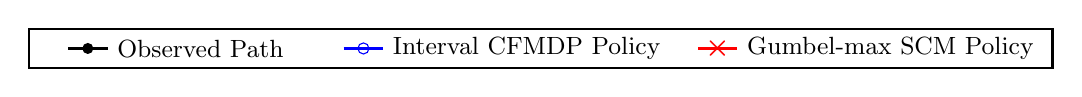
\begin{tikzpicture}[scale=1.0, every node/.style={scale=1.0}]
            \draw[thick, black] (-3, -0.25) rectangle (10, 0.25);
            %
            \draw[black, line width=1pt] (-2.5, 0.0) -- (-2,0.0);
            \fill[black] (-2.25,0.0) circle (2pt); %
            \node[right] at (-2,0.0) {\small Observed Path};
            
            %
            \draw[blue, line width=1pt] (1.0,0.0) -- (1.5,0.0);
            \node[draw=blue, circle, minimum size=4pt, inner sep=0pt] at (1.25,0.0) {}; %
            \node[right] at (1.5,0.0) {\small Interval CFMDP Policy};
            
            %
            \draw[red, line width=1pt] (5.5,0) -- (6,0);
            \node[red] at (5.75,0) {$\boldsymbol{\times}$}; %
            \node[right] at (6,0) {\small Gumbel-max SCM Policy};
        \end{tikzpicture}
    }\\
    %
    \subfigure[\footnotesize Lowest cumulative reward: Interval CFMDP ($312$), Gumbel-max SCM ($312$)]{%
        \resizebox{0.76\columnwidth}{!}{
             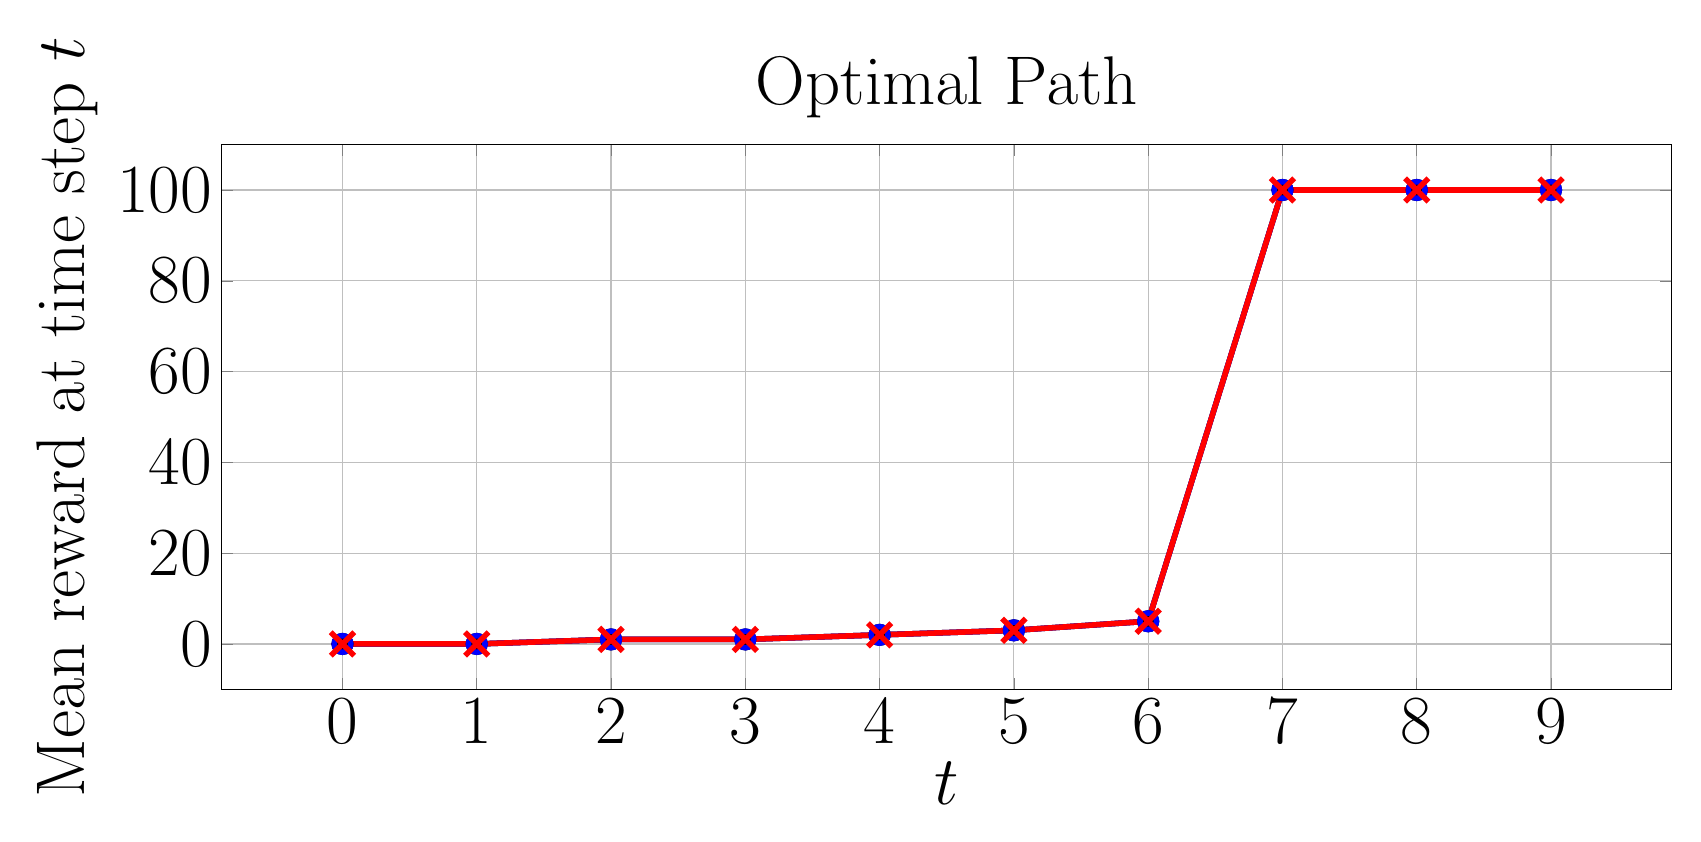
\begin{tikzpicture}
                \begin{axis}[
                    xlabel={$t$},
                    ylabel={Mean reward at time step $t$},
                    title={Optimal Path},
                    grid=both,
                    width=20cm, height=8.5cm,
                    every axis/.style={font=\Huge},
                    %
                ]
                \addplot[
                    color=black, %
                    mark=*, %
                    line width=2pt,
                    mark size=3pt,
                    error bars/.cd,
                    y dir=both, %
                    y explicit, %
                    error bar style={line width=1pt,solid},
                    error mark options={line width=1pt,mark size=4pt,rotate=90}
                ]
                coordinates {
                    (0, 0.0)  +- (0, 0.0)
                    (1, 0.0)  +- (0, 0.0) 
                    (2, 1.0)  +- (0, 0.0) 
                    (3, 1.0)  +- (0, 0.0)
                    (4, 2.0)  +- (0, 0.0)
                    (5, 3.0) +- (0, 0.0)
                    (6, 5.0) +- (0, 0.0)
                    (7, 100.0) +- (0, 0.0)
                    (8, 100.0) +- (0, 0.0)
                    (9, 100.0) +- (0, 0.0)
                };
                %
                \addplot[
                    color=blue, %
                    mark=o, %
                    line width=2pt,
                    mark size=3pt,
                    error bars/.cd,
                    y dir=both, %
                    y explicit, %
                    error bar style={line width=1pt,solid},
                    error mark options={line width=1pt,mark size=4pt,rotate=90}
                ]
                 coordinates {
                    (0, 0.0)  +- (0, 0.0)
                    (1, 0.0)  +- (0, 0.0) 
                    (2, 1.0)  +- (0, 0.0) 
                    (3, 1.0)  +- (0, 0.0)
                    (4, 2.0)  +- (0, 0.0)
                    (5, 3.0) +- (0, 0.0)
                    (6, 5.0) +- (0, 0.0)
                    (7, 100.0) +- (0, 0.0)
                    (8, 100.0) +- (0, 0.0)
                    (9, 100.0) +- (0, 0.0)
                };
                %
                \addplot[
                    color=red, %
                    mark=x, %
                    line width=2pt,
                    mark size=6pt,
                    error bars/.cd,
                    y dir=both, %
                    y explicit, %
                    error bar style={line width=1pt,solid},
                    error mark options={line width=1pt,mark size=4pt,rotate=90}
                ]
                coordinates {
                    (0, 0.0)  +- (0, 0.0)
                    (1, 0.0)  +- (0, 0.0) 
                    (2, 1.0)  +- (0, 0.0) 
                    (3, 1.0)  +- (0, 0.0)
                    (4, 2.0)  +- (0, 0.0)
                    (5, 3.0) +- (0, 0.0)
                    (6, 5.0) +- (0, 0.0)
                    (7, 100.0) +- (0, 0.0)
                    (8, 100.0) +- (0, 0.0)
                    (9, 100.0) +- (0, 0.0)
                };
                \end{axis}
            \end{tikzpicture}
         }
    }
    \hspace{1cm}
    \subfigure[\footnotesize Lowest cumulative reward: Interval CFMDP ($19$), Gumbel-max SCM ($-88$)]{%
         \resizebox{0.76\columnwidth}{!}{
            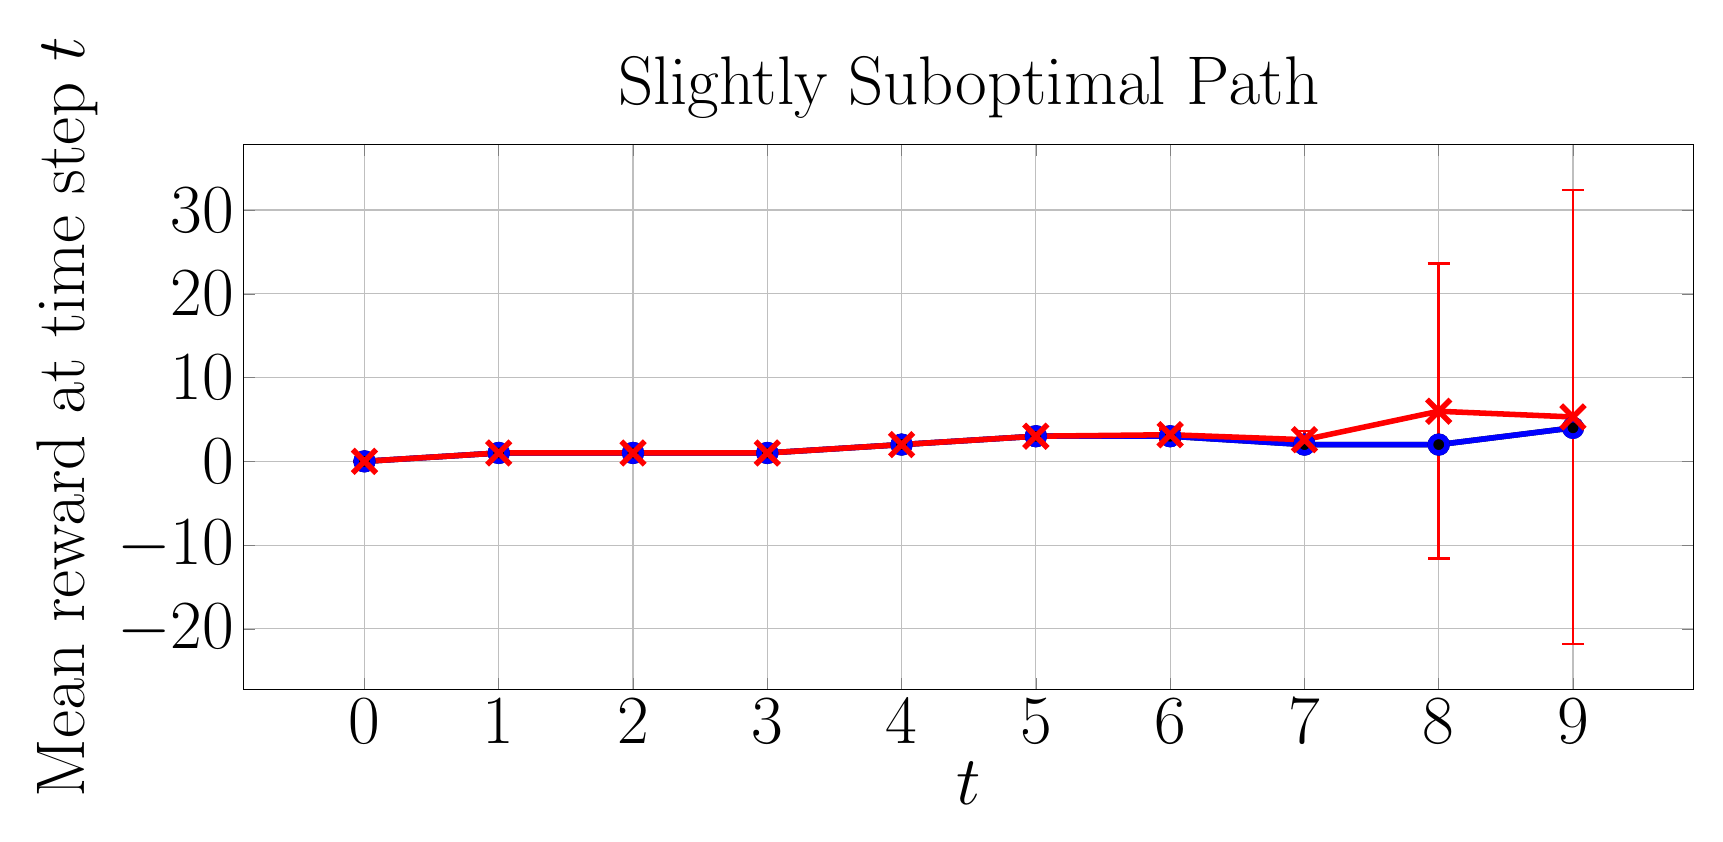
\begin{tikzpicture}
                \begin{axis}[
                    xlabel={$t$},
                    ylabel={Mean reward at time step $t$},
                    title={Slightly Suboptimal Path},
                    grid=both,
                    width=20cm, height=8.5cm,
                    every axis/.style={font=\Huge},
                    %
                ]
                \addplot[
                    color=black, %
                    mark=*, %
                    line width=2pt,
                    mark size=3pt,
                    error bars/.cd,
                    y dir=both, %
                    y explicit, %
                    error bar style={line width=1pt,solid},
                    error mark options={line width=1pt,mark size=4pt,rotate=90}
                ]
              coordinates {
                    (0, 0.0)  +- (0, 0.0)
                    (1, 1.0)  +- (0, 0.0) 
                    (2, 1.0)  +- (0, 0.0) 
                    (3, 1.0)  +- (0, 0.0)
                    (4, 2.0)  +- (0, 0.0)
                    (5, 3.0) +- (0, 0.0)
                    (6, 3.0) +- (0, 0.0)
                    (7, 2.0) +- (0, 0.0)
                    (8, 2.0) +- (0, 0.0)
                    (9, 4.0) +- (0, 0.0)
                };
                %
                \addplot[
                    color=blue, %
                    mark=o, %
                    line width=2pt,
                    mark size=3pt,
                    error bars/.cd,
                    y dir=both, %
                    y explicit, %
                    error bar style={line width=1pt,solid},
                    error mark options={line width=1pt,mark size=4pt,rotate=90}
                ]
              coordinates {
                    (0, 0.0)  +- (0, 0.0)
                    (1, 1.0)  +- (0, 0.0) 
                    (2, 1.0)  +- (0, 0.0) 
                    (3, 1.0)  +- (0, 0.0)
                    (4, 2.0)  +- (0, 0.0)
                    (5, 3.0) +- (0, 0.0)
                    (6, 3.0) +- (0, 0.0)
                    (7, 2.0) +- (0, 0.0)
                    (8, 2.0) +- (0, 0.0)
                    (9, 4.0) +- (0, 0.0)
                };
                %
                \addplot[
                    color=red, %
                    mark=x, %
                    line width=2pt,
                    mark size=6pt,
                    error bars/.cd,
                    y dir=both, %
                    y explicit, %
                    error bar style={line width=1pt,solid},
                    error mark options={line width=1pt,mark size=4pt,rotate=90}
                ]
                coordinates {
                    (0, 0.0)  +- (0, 0.0)
                    (1, 1.0)  +- (0, 0.0) 
                    (2, 1.0)  +- (0, 0.0) 
                    (3, 1.0)  +- (0, 0.0)
                    (4, 2.0)  += (0, 0.0)
                    (5, 3.0)  += (0, 0.0)
                    (6, 3.17847) += (0, 0.62606746) -= (0, 0.62606746)
                    (7, 2.5832885) += (0, 1.04598233) -= (0, 1.04598233)
                    (8, 5.978909) += (0, 17.60137623) -= (0, 17.60137623)
                    (9, 5.297059) += (0, 27.09227512) -= (0, 27.09227512)
                };
                \end{axis}
            \end{tikzpicture}
         }
    }\\[-1.5pt]
    \subfigure[\footnotesize Lowest cumulative reward: Interval CFMDP ($14$), Gumbel-max SCM ($-598$)]{%
         \resizebox{0.76\columnwidth}{!}{
             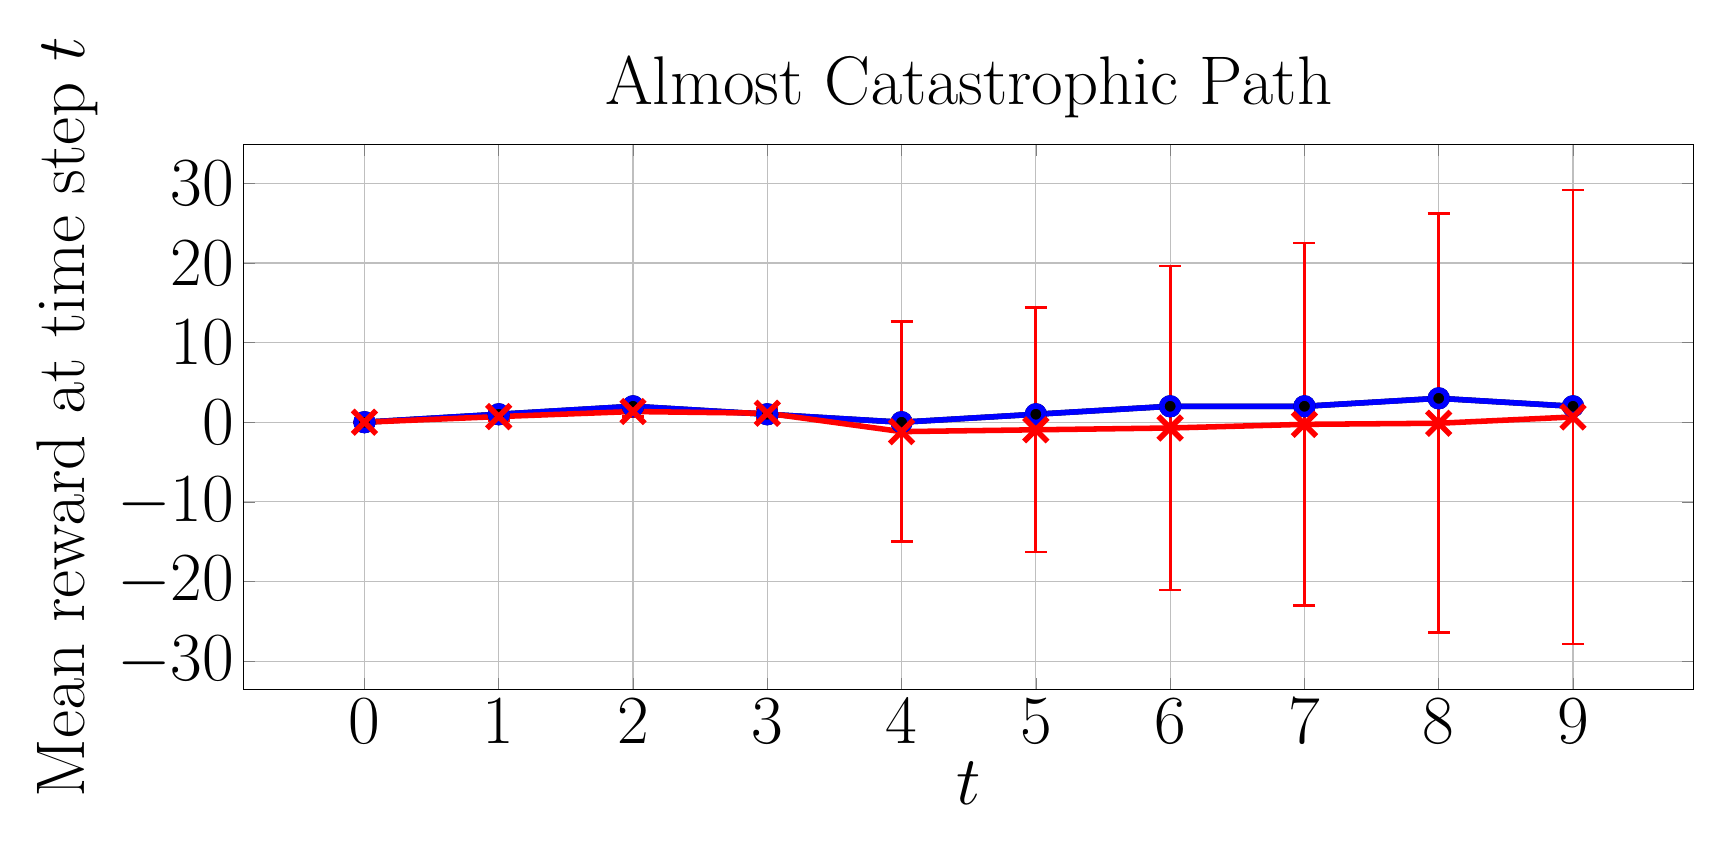
\begin{tikzpicture}
                \begin{axis}[
                    xlabel={$t$},
                    ylabel={Mean reward at time step $t$},
                    title={Almost Catastrophic Path},
                    grid=both,
                    width=20cm, height=8.5cm,
                    every axis/.style={font=\Huge},
                    %
                ]
                \addplot[
                    color=black, %
                    mark=*, %
                    line width=2pt,
                    mark size=3pt,
                    error bars/.cd,
                    y dir=both, %
                    y explicit, %
                    error bar style={line width=1pt,solid},
                    error mark options={line width=1pt,mark size=4pt,rotate=90}
                ]
                coordinates {
                    (0, 0.0)  +- (0, 0.0)
                    (1, 1.0)  +- (0, 0.0) 
                    (2, 2.0)  +- (0, 0.0) 
                    (3, 1.0)  +- (0, 0.0)
                    (4, 0.0)  +- (0, 0.0)
                    (5, 1.0) +- (0, 0.0)
                    (6, 2.0) +- (0, 0.0)
                    (7, 2.0) +- (0, 0.0)
                    (8, 3.0) +- (0, 0.0)
                    (9, 2.0) +- (0, 0.0)
                };
                %
                \addplot[
                    color=blue, %
                    mark=o, %
                    line width=2pt,
                    mark size=3pt,
                    error bars/.cd,
                    y dir=both, %
                    y explicit, %
                    error bar style={line width=1pt,solid},
                    error mark options={line width=1pt,mark size=4pt,rotate=90}
                ]
                coordinates {
                    (0, 0.0)  +- (0, 0.0)
                    (1, 1.0)  +- (0, 0.0) 
                    (2, 2.0)  +- (0, 0.0) 
                    (3, 1.0)  +- (0, 0.0)
                    (4, 0.0)  +- (0, 0.0)
                    (5, 1.0) +- (0, 0.0)
                    (6, 2.0) +- (0, 0.0)
                    (7, 2.0) +- (0, 0.0)
                    (8, 3.0) +- (0, 0.0)
                    (9, 2.0) +- (0, 0.0)
                };
                %
                \addplot[
                    color=red, %
                    mark=x, %
                    line width=2pt,
                    mark size=6pt,
                    error bars/.cd,
                    y dir=both, %
                    y explicit, %
                    error bar style={line width=1pt,solid},
                    error mark options={line width=1pt,mark size=4pt,rotate=90}
                ]
                coordinates {
                    (0, 0.0)  +- (0, 0.0)
                    (1, 0.7065655)  +- (0, 0.4553358) 
                    (2, 1.341673)  +- (0, 0.67091621) 
                    (3, 1.122926)  +- (0, 0.61281824)
                    (4, -1.1821935)  +- (0, 13.82444042)
                    (5, -0.952399)  +- (0, 15.35195457)
                    (6, -0.72672) +- (0, 20.33508414)
                    (7, -0.268983) +- (0, 22.77861454)
                    (8, -0.1310835) +- (0, 26.31013314)
                    (9, 0.65806) +- (0, 28.50670214)
                };
                %
            %
            %
            %
            %
            %
            %
            %
            %
            %
            %
            %
            %
            %
            %
            %
            %
            %
            %
                \end{axis}
            \end{tikzpicture}
         }
    }
    \hspace{1cm}
    \subfigure[\footnotesize Lowest cumulative reward: Interval CFMDP ($-698$), Gumbel-max SCM ($-698$)]{%
         \resizebox{0.76\columnwidth}{!}{
            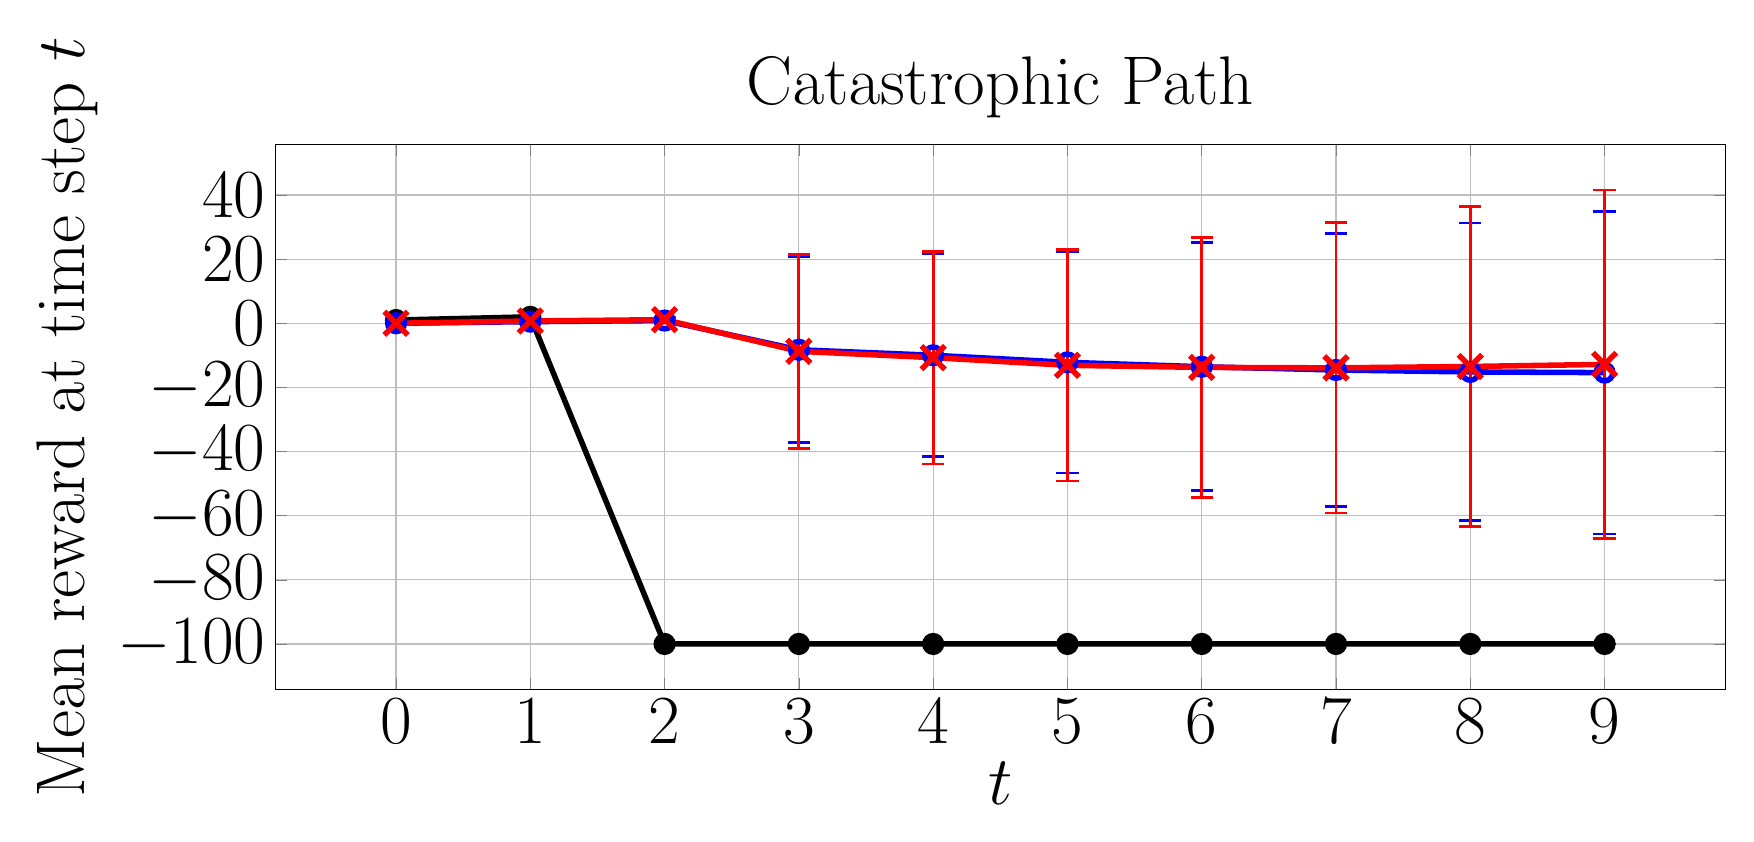
\begin{tikzpicture}
                \begin{axis}[
                    xlabel={$t$},
                    ylabel={Mean reward at time step $t$},
                    title={Catastrophic Path},
                    grid=both,
                    width=20cm, height=8.5cm,
                    every axis/.style={font=\Huge},
                    %
                ]
                \addplot[
                    color=black, %
                    mark=*, %
                    line width=2pt,
                    mark size=3pt,
                    error bars/.cd,
                    y dir=both, %
                    y explicit, %
                    error bar style={line width=1pt,solid},
                    error mark options={line width=1pt,mark size=4pt,rotate=90}
                ]
                coordinates {
                    (0, 1.0)  +- (0, 0.0)
                    (1, 2.0)  +- (0, 0.0) 
                    (2, -100.0)  +- (0, 0.0) 
                    (3, -100.0)  +- (0, 0.0)
                    (4, -100.0)  +- (0, 0.0)
                    (5, -100.0) +- (0, 0.0)
                    (6, -100.0) +- (0, 0.0)
                    (7, -100.0) +- (0, 0.0)
                    (8, -100.0) +- (0, 0.0)
                    (9, -100.0) +- (0, 0.0)
                };
                %
                \addplot[
                    color=blue, %
                    mark=o, %
                    line width=2pt,
                    mark size=3pt,
                    error bars/.cd,
                    y dir=both, %
                    y explicit, %
                    error bar style={line width=1pt,solid},
                    error mark options={line width=1pt,mark size=4pt,rotate=90}
                ]
                coordinates {
                    (0, 0.0)  +- (0, 0.0)
                    (1, 0.504814)  +- (0, 0.49997682) 
                    (2, 0.8439835)  +- (0, 0.76831917) 
                    (3, -8.2709165)  +- (0, 28.93656754)
                    (4, -9.981082)  +- (0, 31.66825363)
                    (5, -12.1776325) +- (0, 34.53463233)
                    (6, -13.556076) +- (0, 38.62845372)
                    (7, -14.574418) +- (0, 42.49603359)
                    (8, -15.1757075) +- (0, 46.41913968)
                    (9, -15.3900395) +- (0, 50.33563368)
                };
                %
                \addplot[
                    color=red, %
                    mark=x, %
                    line width=2pt,
                    mark size=6pt,
                    error bars/.cd,
                    y dir=both, %
                    y explicit, %
                    error bar style={line width=1pt,solid},
                    error mark options={line width=1pt,mark size=4pt,rotate=90}
                ]
                coordinates {
                    (0, 0.0)  +- (0, 0.0)
                    (1, 0.701873)  +- (0, 0.45743556) 
                    (2, 1.1227805)  +- (0, 0.73433129) 
                    (3, -8.7503255)  +- (0, 30.30257976)
                    (4, -10.722092)  +- (0, 33.17618589)
                    (5, -13.10721)  +- (0, 36.0648089)
                    (6, -13.7631645) +- (0, 40.56553451)
                    (7, -13.909043) +- (0, 45.23829402)
                    (8, -13.472517) +- (0, 49.96270296)
                    (9, -12.8278835) +- (0, 54.38618735)
                };
                %
            %
            %
            %
            %
            %
            %
            %
            %
            %
            %
            %
            %
            %
            %
            %
            %
            %
            %
                \end{axis}
            \end{tikzpicture}
         }
    }
    \caption{Average instant reward of CF paths induced by policies on GridWorld $p=0.4$.}
    \label{fig: reward p=0.4}
\end{figure*}

\subsection{Experimental Setup}
To compare policy performance, we measure the average rewards of counterfactual paths induced by our policy and the Gumbel-max policy by uniformly sampling $200$ counterfactual MDPs from the ICFMDP and generating $10,000$ counterfactual paths over each sampled CFMDP. \jl{Since the interval CFMDP depends on the observed path, we select $4$  paths of varying optimality to evaluate how the observed path impacts the performance of both policies: an optimal path, a slightly suboptimal path that could reach the optimal reward with a few changes, a catastrophic path that enters a catastrophic, terminal state with low reward, and an almost catastrophic path that was close to entering a catastrophic state.} When measuring the average probability bound widths and execution time needed to generate the ICFMDPs, we averaged over $20$ randomly generated observed paths
\footnote{Further training details are provided in Appendix \ref{app: training details}, and the code is provided at \href{https://github.com/ddv-lab/robust-cf-inference-in-MDPs}{https://github.com/ddv-lab/robust-cf-inference-in-MDPs}
%
%
.}.

\subsection{GridWorld}
\jl{The GridWorld MDP is a $4 \times 4$ grid where an agent must navigate from the top-left corner to the goal state in the bottom-right corner, avoiding a dangerous terminal state in the centre. At each time step, the agent can move up, down, left, or right, but there is a small probability (controlled by hyper-parameter $p$) of moving in an unintended direction. As the agent nears the goal, the reward for each state increases, culminating in a reward of $+100$ for reaching the goal. Entering the dangerous state results in a penalty of $-100$. We use two versions of GridWorld: a less stochastic version with $p=0.9$ (i.e., $90$\% chance of moving in the chosen direction) and a more stochastic version with $p=0.4$.}

\paragraph{GridWorld ($p=0.9$)}
When $p=0.9$, the counterfactual probability bounds are typically narrow (see Table \ref{tab:nonzero_probs} for average measurements). Consequently, as shown in Figure \ref{fig: reward p=0.9}, both policies are nearly identical and perform similarly well across the optimal, slightly suboptimal, and catastrophic paths.
%
However, for the almost catastrophic path, the interval CFMDP path is more conservative and follows the observed path more closely (as this is where the probability bounds are narrowest), which typically requires one additional step to reach the goal state than the Gumbel-max SCM policy.
%

\paragraph{GridWorld ($p=0.4$)}
\jl{When $p=0.4$, the GridWorld environment becomes more uncertain, increasing the risk of entering the dangerous state even if correct actions are chosen. Thus, as shown in Figure \ref{fig: reward p=0.4}, the interval CFMDP policy adopts a more conservative approach, avoiding deviation from the observed policy if it cannot guarantee higher counterfactual rewards (see the slightly suboptimal and almost catastrophic paths), whereas the Gumbel-max SCM is inconsistent: it can yield higher rewards, but also much lower rewards, reflected in the wide error bars.} For the catastrophic path, both policies must deviate from the observed path to achieve a higher reward and, in this case, perform similarly.
%
%
%
%
\subsection{Sepsis}
The Sepsis MDP \citep{oberst2019counterfactual} simulates trajectories of Sepsis patients. Each state consists of four vital signs (heart rate, blood pressure, oxygen concentration, and glucose levels), categorised as low, normal, or high.
and three treatments that can be toggled on/off at each time step (8 actions in total). Unlike \citet{oberst2019counterfactual}, we scale rewards based on the number of out-of-range vital signs, between $-1000$ (patient dies) and $1000$ (patient discharged). \jl{Like the GridWorld $p=0.4$ experiment, the Sepsis MDP is highly uncertain, as many states are equally likely to lead to optimal and poor outcomes. Thus, as shown in Figure \ref{fig: reward sepsis}, both policies follow the observed optimal and almost catastrophic paths to guarantee rewards are no worse than the observation.} However, improving the catastrophic path requires deviating from the observation. Here, the Gumbel-max SCM policy, on average, performs better than the interval CFMDP policy. But, since both policies have lower bounds clipped at $-1000$, neither policy reliably improves over the observation. In contrast, for the slightly suboptimal path, the interval CFMDP policy performs significantly better, shown by its higher lower bounds. 
Moreover, in these two cases, the worst-case counterfactual path generated by the interval CFMDP policy is better than that of the Gumbel-max SCM policy,
indicating its greater robustness.
%
\begin{figure*}
    \centering
     \resizebox{0.6\textwidth}{!}{
        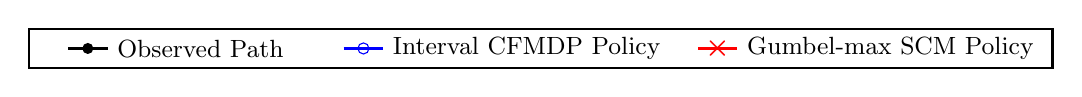
\begin{tikzpicture}[scale=1.0, every node/.style={scale=1.0}]
            \draw[thick, black] (-3, -0.25) rectangle (10, 0.25);
            %
            \draw[black, line width=1pt] (-2.5, 0.0) -- (-2,0.0);
            \fill[black] (-2.25,0.0) circle (2pt); %
            \node[right] at (-2,0.0) {\small Observed Path};
            
            %
            \draw[blue, line width=1pt] (1.0,0.0) -- (1.5,0.0);
            \node[draw=blue, circle, minimum size=4pt, inner sep=0pt] at (1.25,0.0) {}; %
            \node[right] at (1.5,0.0) {\small Interval CFMDP Policy};
            
            %
            \draw[red, line width=1pt] (5.5,0) -- (6,0);
            \node[red] at (5.75,0) {$\boldsymbol{\times}$}; %
            \node[right] at (6,0) {\small Gumbel-max SCM Policy};
        \end{tikzpicture}
    }\\
    \subfigure[\footnotesize Lowest cumulative reward: Interval CFMDP ($8000$), Gumbel-max SCM ($8000$)]{%
         \resizebox{0.76\columnwidth}{!}{
             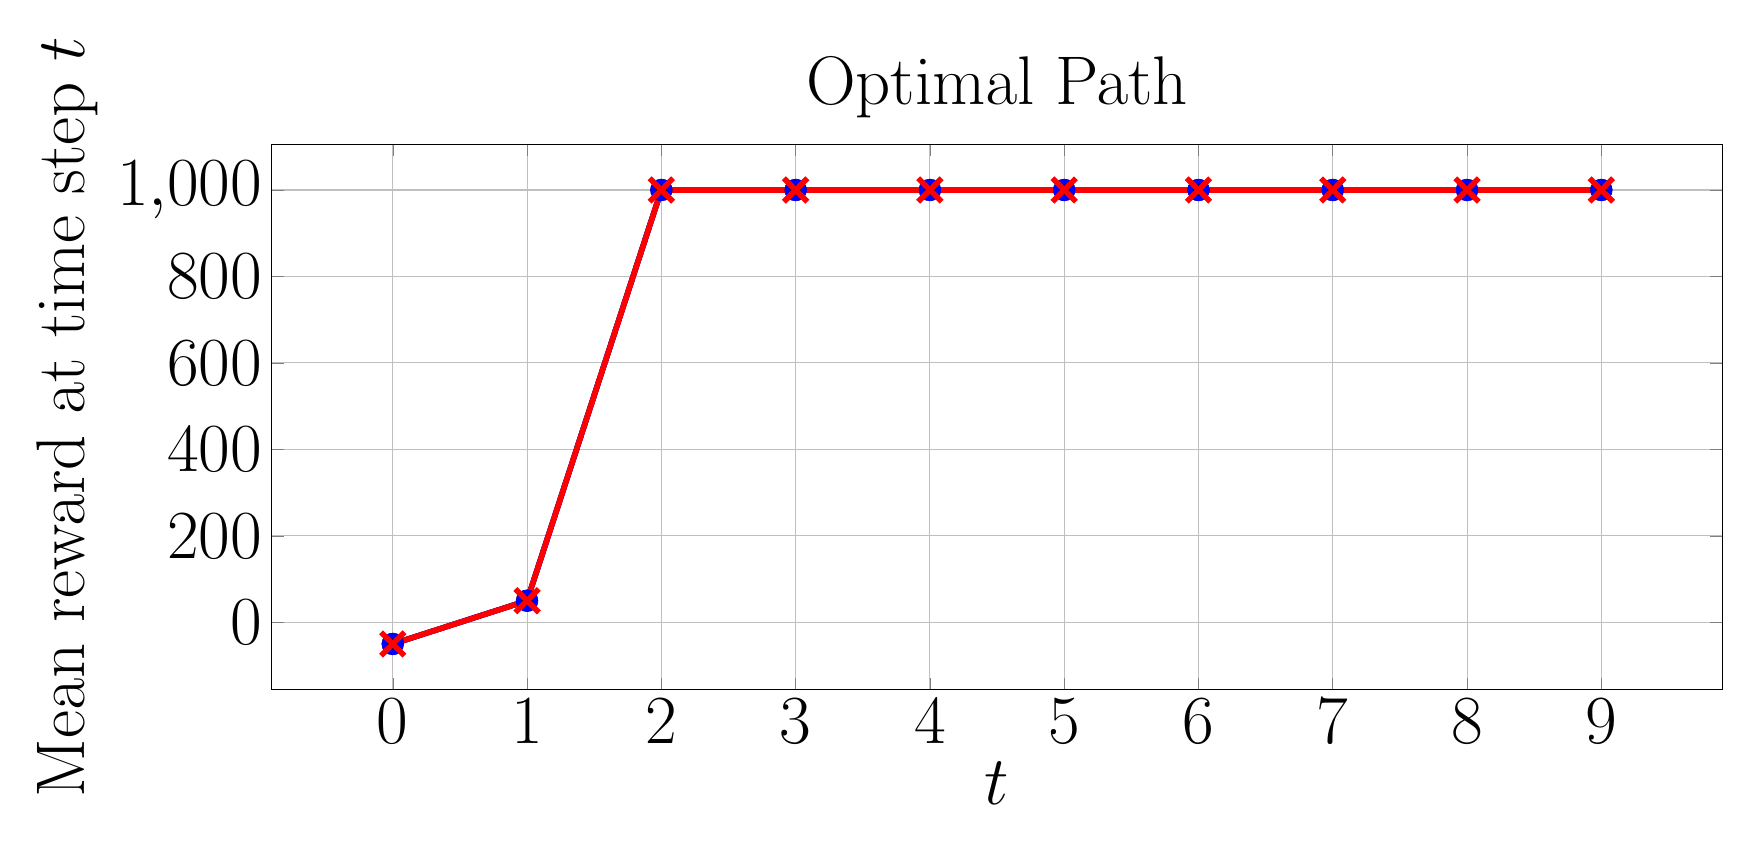
\begin{tikzpicture}
                \begin{axis}[
                    xlabel={$t$},
                    ylabel={Mean reward at time step $t$},
                    title={Optimal Path},
                    grid=both,
                    width=20cm, height=8.5cm,
                    every axis/.style={font=\Huge},
                    %
                ]
                \addplot[
                    color=black, %
                    mark=*, %
                    line width=2pt,
                    mark size=3pt,
                ]
                coordinates {
                    (0, -50.0)
                    (1, 50.0)
                    (2, 1000.0)
                    (3, 1000.0)
                    (4, 1000.0)
                    (5, 1000.0)
                    (6, 1000.0)
                    (7, 1000.0)
                    (8, 1000.0)
                    (9, 1000.0)
                };
                %
                \addplot[
                    color=blue, %
                    mark=o, %
                    line width=2pt,
                    mark size=3pt,
                    error bars/.cd,
                    y dir=both, %
                    y explicit, %
                    error bar style={line width=1pt,solid},
                    error mark options={line width=1pt,mark size=4pt,rotate=90}
                ]
                coordinates {
                    (0, -50.0)  +- (0, 0.0)
                    (1, 50.0)  +- (0, 0.0) 
                    (2, 1000.0)  +- (0, 0.0) 
                    (3, 1000.0)  +- (0, 0.0)
                    (4, 1000.0)  +- (0, 0.0)
                    (5, 1000.0) +- (0, 0.0)
                    (6, 1000.0) +- (0, 0.0)
                    (7, 1000.0) +- (0, 0.0)
                    (8, 1000.0) +- (0, 0.0)
                    (9, 1000.0) +- (0, 0.0)
                };
                %
                \addplot[
                    color=red, %
                    mark=x, %
                    line width=2pt,
                    mark size=6pt,
                    error bars/.cd,
                    y dir=both, %
                    y explicit, %
                    error bar style={line width=1pt,solid},
                    error mark options={line width=1pt,mark size=4pt,rotate=90}
                ]
                coordinates {
                    (0, -50.0)  +- (0, 0.0)
                    (1, 50.0)  +- (0, 0.0) 
                    (2, 1000.0)  +- (0, 0.0) 
                    (3, 1000.0)  +- (0, 0.0)
                    (4, 1000.0)  +- (0, 0.0)
                    (5, 1000.0) +- (0, 0.0)
                    (6, 1000.0) +- (0, 0.0)
                    (7, 1000.0) +- (0, 0.0)
                    (8, 1000.0) +- (0, 0.0)
                    (9, 1000.0) +- (0, 0.0)
                };
                %
                \end{axis}
            \end{tikzpicture}
         }
    }
    \hspace{1cm}
    \subfigure[\footnotesize Lowest cumulative reward: Interval CFMDP ($-5980$), Gumbel-max SCM ($-8000$)]{%
         \resizebox{0.76\columnwidth}{!}{
            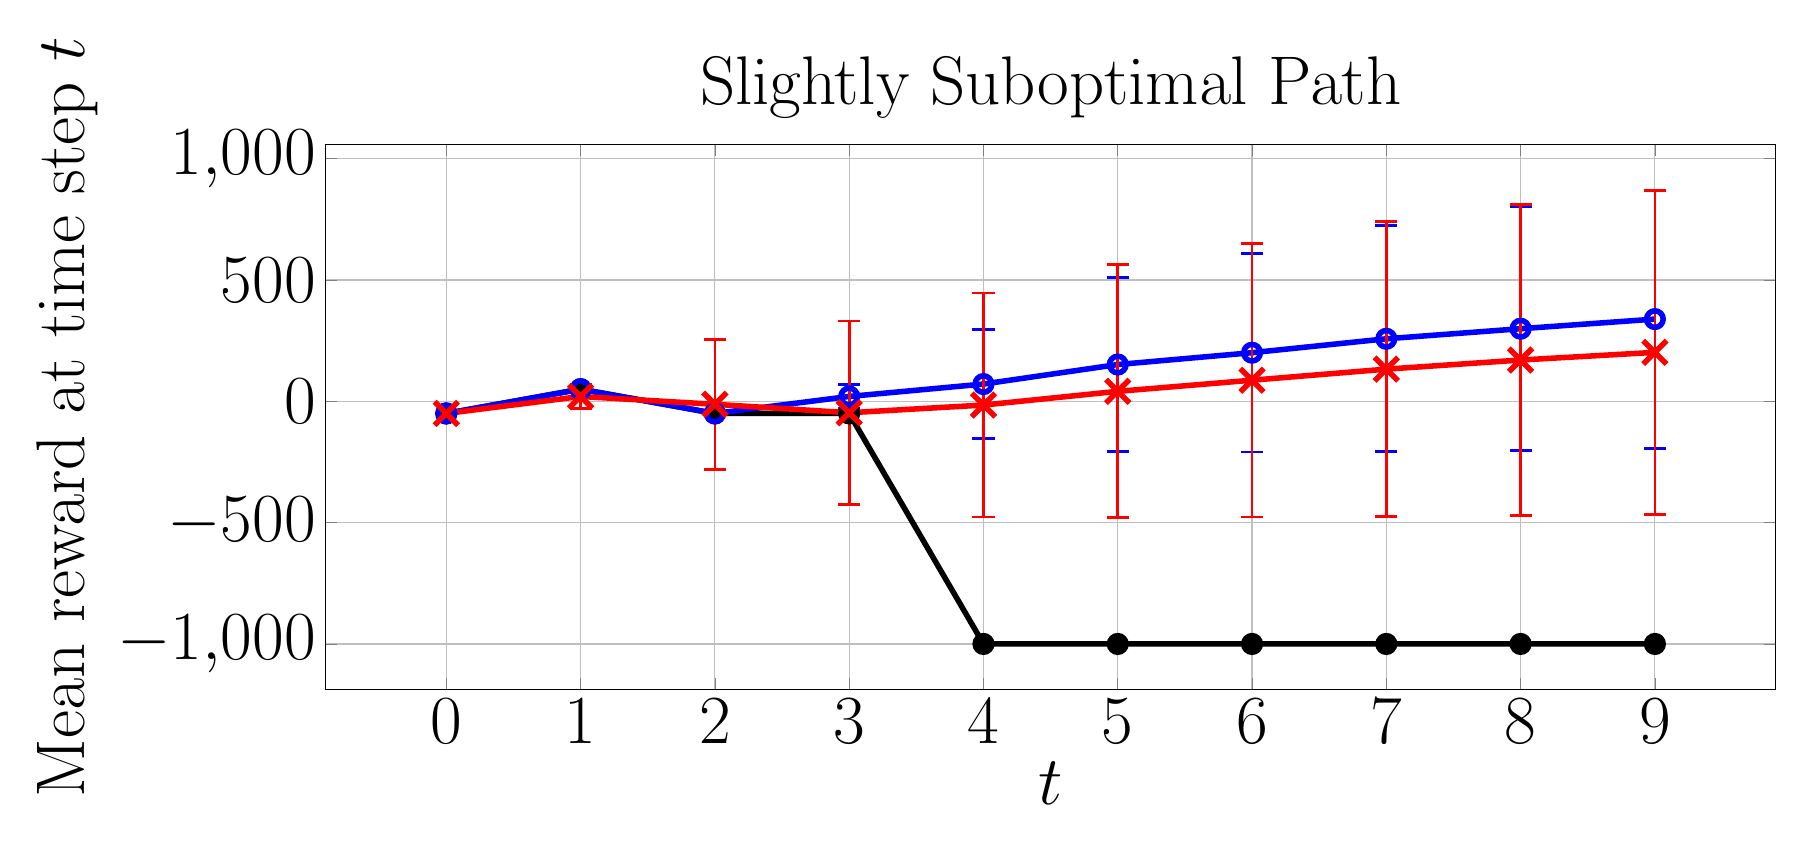
\begin{tikzpicture}
                \begin{axis}[
                    xlabel={$t$},
                    ylabel={Mean reward at time step $t$},
                    title={Slightly Suboptimal Path},
                    grid=both,
                    width=20cm, height=8.5cm,
                    every axis/.style={font=\Huge},
                    %
                ]
               \addplot[
                    color=black, %
                    mark=*, %
                    line width=2pt,
                    mark size=3pt,
                ]
                coordinates {
                    (0, -50.0)
                    (1, 50.0)
                    (2, -50.0)
                    (3, -50.0)
                    (4, -1000.0)
                    (5, -1000.0)
                    (6, -1000.0)
                    (7, -1000.0)
                    (8, -1000.0)
                    (9, -1000.0)
                };
                %
                \addplot[
                    color=blue, %
                    mark=o, %
                    line width=2pt,
                    mark size=3pt,
                    error bars/.cd,
                    y dir=both, %
                    y explicit, %
                    error bar style={line width=1pt,solid},
                    error mark options={line width=1pt,mark size=4pt,rotate=90}
                ]
                coordinates {
                    (0, -50.0)  +- (0, 0.0)
                    (1, 50.0)  +- (0, 0.0) 
                    (2, -50.0)  +- (0, 0.0) 
                    (3, 20.0631)  +- (0, 49.97539413)
                    (4, 71.206585)  +- (0, 226.02033693)
                    (5, 151.60797) +- (0, 359.23292559)
                    (6, 200.40593) +- (0, 408.86185176)
                    (7, 257.77948) +- (0, 466.10372804)
                    (8, 299.237465) +- (0, 501.82579506)
                    (9, 338.9129) +- (0, 532.06124996)
                };
                %
                \addplot[
                    color=red, %
                    mark=x, %
                    line width=2pt,
                    mark size=6pt,
                    error bars/.cd,
                    y dir=both, %
                    y explicit, %
                    error bar style={line width=1pt,solid},
                    error mark options={line width=1pt,mark size=4pt,rotate=90}
                ]
                coordinates {
                    (0, -50.0)  +- (0, 0.0)
                    (1, 20.00736)  +- (0, 49.99786741) 
                    (2, -12.282865)  +- (0, 267.598755) 
                    (3, -47.125995)  +- (0, 378.41755832)
                    (4, -15.381965)  +- (0, 461.77616558)
                    (5, 41.15459) +- (0, 521.53189262)
                    (6, 87.01595) +- (0, 564.22243126 )
                    (7, 132.62376) +- (0, 607.31338037)
                    (8, 170.168145) +- (0, 641.48013693)
                    (9, 201.813135) +- (0, 667.29441777)
                };
                %
                %
                %
                %
                %
                %
                %
                %
                %
                %
                %
                %
                %
                %
                %
                %
                %
                %
                %
                \end{axis}
            \end{tikzpicture}
         }
    }\\[-1.5pt]
    \subfigure[\footnotesize Lowest cumulative reward: Interval CFMDP ($100$), Gumbel-max SCM ($100$)]{%
         \resizebox{0.76\columnwidth}{!}{
             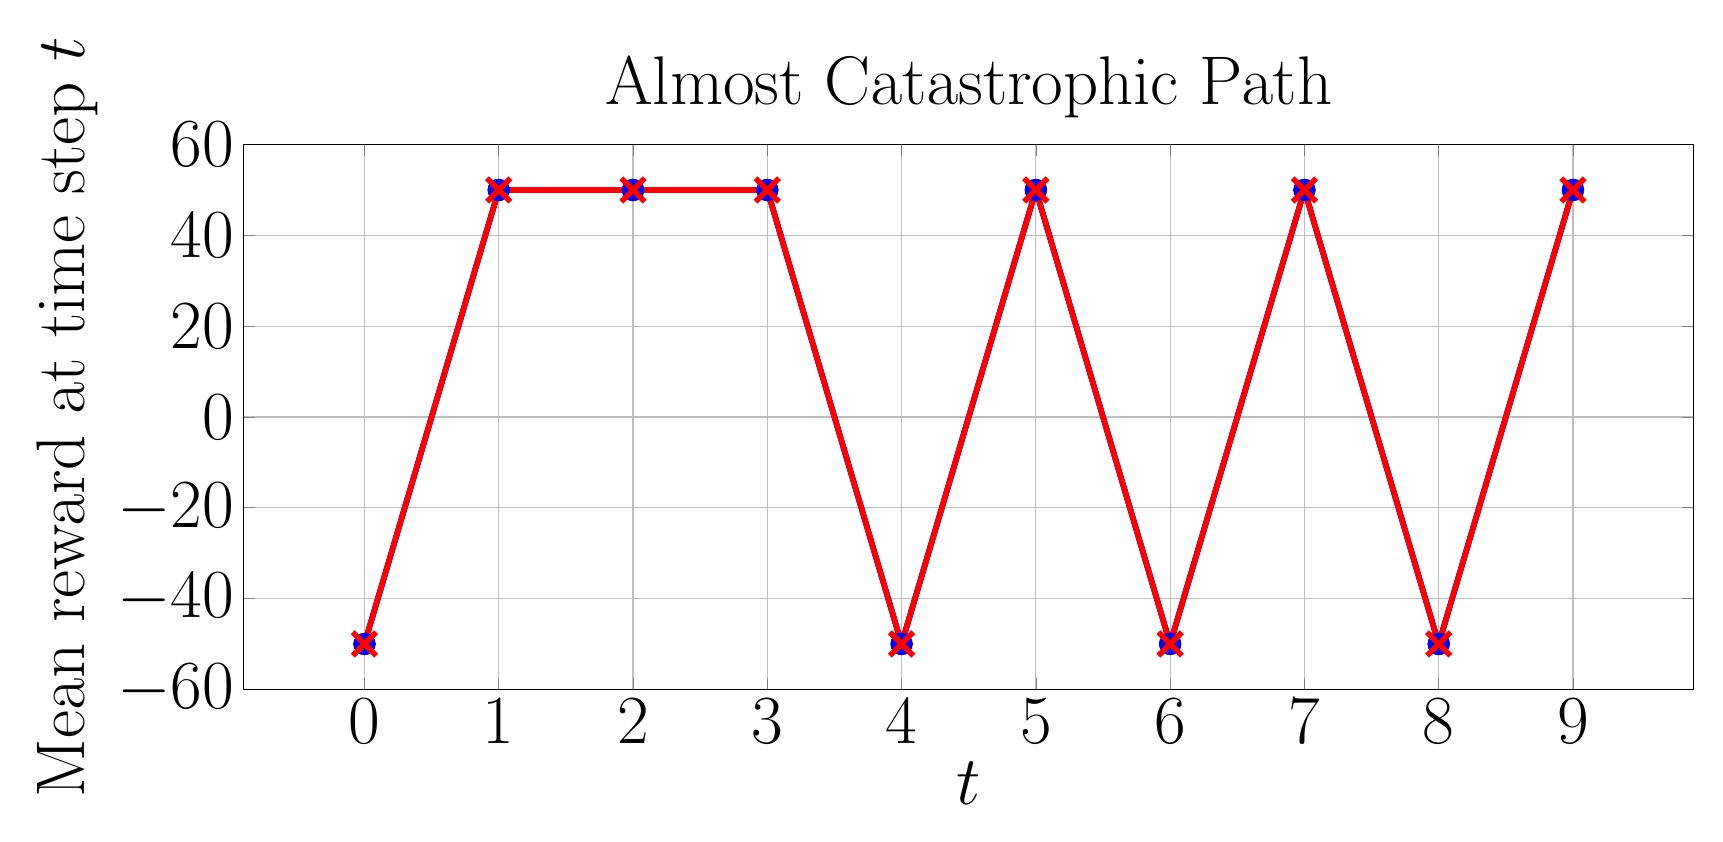
\begin{tikzpicture}
                \begin{axis}[
                    xlabel={$t$},
                    ylabel={Mean reward at time step $t$},
                    title={Almost Catastrophic Path},
                    grid=both,
                    every axis/.style={font=\Huge},
                    width=20cm, height=8.5cm,
                    %
                ]
               \addplot[
                    color=black, %
                    mark=*, %
                    line width=2pt,
                    mark size=3pt,
                ]
                coordinates {
                    (0, -50.0)
                    (1, 50.0)
                    (2, 50.0)
                    (3, 50.0)
                    (4, -50.0)
                    (5, 50.0)
                    (6, -50.0)
                    (7, 50.0)
                    (8, -50.0)
                    (9, 50.0)
                };
                %
                %
                \addplot[
                    color=blue, %
                    mark=o, %
                    line width=2pt,
                    mark size=3pt,
                    error bars/.cd,
                    y dir=both, %
                    y explicit, %
                    error bar style={line width=1pt,solid},
                    error mark options={line width=1pt,mark size=4pt,rotate=90}
                ]
                coordinates {
                    (0, -50.0)  +- (0, 0.0)
                    (1, 50.0)  +- (0, 0.0) 
                    (2, 50.0)  +- (0, 0.0) 
                    (3, 50.0)  +- (0, 0.0)
                    (4, -50.0)  +- (0, 0.0)
                    (5, 50.0) +- (0, 0.0)
                    (6, -50.0) +- (0, 0.0)
                    (7, 50.0) +- (0, 0.0)
                    (8, -50.0) +- (0, 0.0)
                    (9, 50.0) +- (0, 0.0)
                };
                %
                \addplot[
                    color=red, %
                    mark=x, %
                    line width=2pt,
                    mark size=6pt,
                    error bars/.cd,
                    y dir=both, %
                    y explicit, %
                    error bar style={line width=1pt,solid},
                    error mark options={line width=1pt,mark size=4pt,rotate=90}
                ]
                coordinates {
                    (0, -50.0)  +- (0, 0.0)
                    (1, 50.0)  +- (0, 0.0) 
                    (2, 50.0)  +- (0, 0.0) 
                    (3, 50.0)  +- (0, 0.0)
                    (4, -50.0)  +- (0, 0.0)
                    (5, 50.0) +- (0, 0.0)
                    (6, -50.0) +- (0, 0.0)
                    (7, 50.0) +- (0, 0.0)
                    (8, -50.0) +- (0, 0.0)
                    (9, 50.0) +- (0, 0.0)
                };
                %
                %
                %
                %
                %
                %
                %
                %
                %
                %
                %
                %
                %
                %
                %
                %
                %
                %
                %
                \end{axis}
            \end{tikzpicture}
         }
    }
    \hspace{1cm}
    \subfigure[\footnotesize Lowest cumulative reward: Interval CFMDP ($-7150$), Gumbel-max SCM ($-9050$)]{%
         \resizebox{0.76\columnwidth}{!}{
            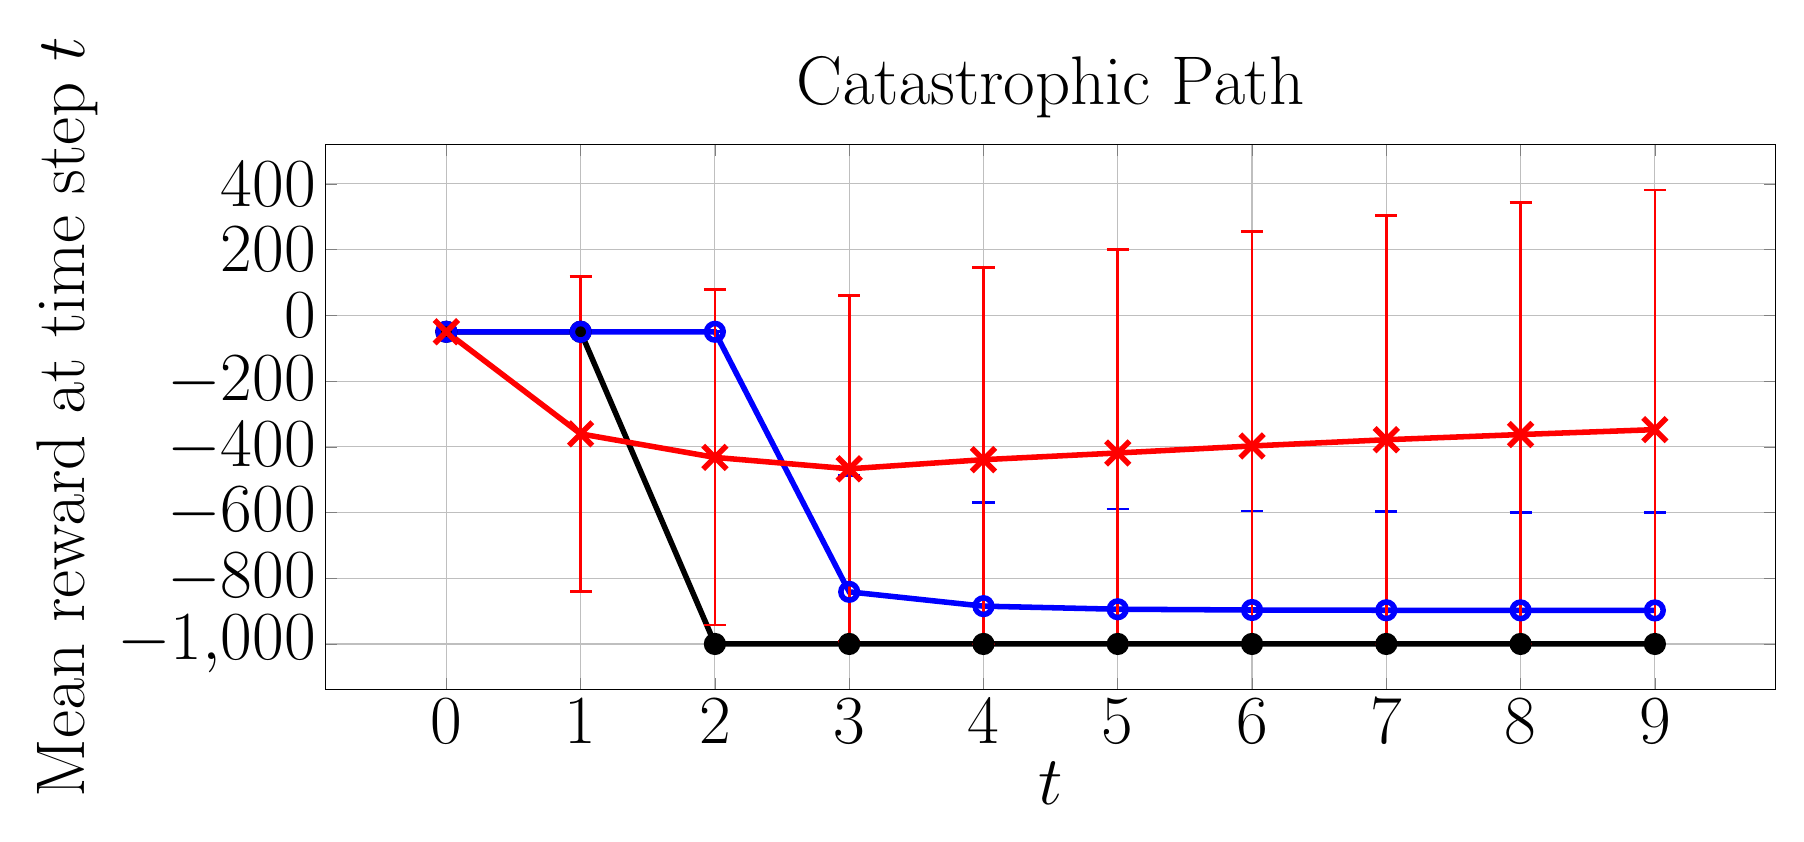
\begin{tikzpicture}
                \begin{axis}[
                    xlabel={$t$},
                    ylabel={Mean reward at time step $t$},
                    title={Catastrophic Path},
                    grid=both,
                    width=20cm, height=8.5cm,
                    every axis/.style={font=\Huge},
                    %
                ]
               \addplot[
                    color=black, %
                    mark=*, %
                    line width=2pt,
                    mark size=3pt,
                ]
                coordinates {
                    (0, -50.0)
                    (1, -50.0)
                    (2, -1000.0)
                    (3, -1000.0)
                    (4, -1000.0)
                    (5, -1000.0)
                    (6, -1000.0)
                    (7, -1000.0)
                    (8, -1000.0)
                    (9, -1000.0)
                };
                %
                %
                \addplot[
                    color=blue, %
                    mark=o, %
                    line width=2pt,
                    mark size=3pt,
                    error bars/.cd,
                    y dir=both, %
                    y explicit, %
                    error bar style={line width=1pt,solid},
                    error mark options={line width=1pt,mark size=4pt,rotate=90}
                ]
                coordinates {
                    (0, -50.0)  +- (0, 0.0)
                    (1, -50.0)  +- (0, 0.0) 
                    (2, -50.0)  +- (0, 0.0) 
                    (3, -841.440725)  += (0, 354.24605512) -= (0, 158.559275)
                    (4, -884.98225)  += (0, 315.37519669) -= (0, 115.01775)
                    (5, -894.330425) += (0, 304.88572805) -= (0, 105.669575)
                    (6, -896.696175) += (0, 301.19954514) -= (0, 103.303825)
                    (7, -897.4635) += (0, 299.61791279) -= (0, 102.5365)
                    (8, -897.77595) += (0, 298.80392585) -= (0, 102.22405)
                    (9, -897.942975) += (0, 298.32920557) -= (0, 102.057025)
                };
                %
                \addplot[
                    color=red, %
                    mark=x, %
                    line width=2pt,
                    mark size=6pt,
                    error bars/.cd,
                    y dir=both, %
                    y explicit, %
                    error bar style={line width=1pt,solid},
                    error mark options={line width=1pt,mark size=4pt,rotate=90}
                ]
            coordinates {
                    (0, -50.0)  +- (0, 0.0)
                    (1, -360.675265)  +- (0, 479.39812699) 
                    (2, -432.27629)  +- (0, 510.38620897) 
                    (3, -467.029545)  += (0, 526.36009628) -= (0, 526.36009628)
                    (4, -439.17429)  += (0, 583.96638919) -= (0, 560.82571)
                    (5, -418.82704) += (0, 618.43027478) -= (0, 581.17296)
                    (6, -397.464895) += (0, 652.67322574) -= (0, 602.535105)
                    (7, -378.49052) += (0, 682.85407033) -= (0, 621.50948)
                    (8, -362.654195) += (0, 707.01412023) -= (0, 637.345805)
                    (9, -347.737935) += (0, 729.29076479) -= (0, 652.262065)
                };
                %
                %
                %
                %
                %
                %
                %
                %
                %
                %
                %
                %
                %
                %
                %
                %
                %
                %
                %
                \end{axis}
            \end{tikzpicture}
         }
    }
    \caption{Average instant reward of CF paths induced by policies on Sepsis.}
    \label{fig: reward sepsis}
\end{figure*}

%
%
%
\subsection{Interval CFMDP Bounds}
%
%
Table \ref{tab:nonzero_probs} presents the mean counterfactual probability bound widths (excluding transitions where the upper bound is $0$) for each MDP, averaged over 20 observed paths. We compare the bounds under counterfactual stability (CS) and monotonicity (M) assumptions, CS alone, and no assumptions. This shows that the assumptions marginally reduce the bound widths, indicating the assumptions tighten the bounds without excluding too many causal models, as intended.
\renewcommand{\arraystretch}{1}

\begin{table}
\centering
\caption{Mean width of counterfactual probability bounds}
\resizebox{0.8\columnwidth}{!}{%
\begin{tabular}{|c|c|c|c|}
\hline
\multirow{2}{*}{\textbf{Environment}} & \multicolumn{3}{c|}{\textbf{Assumptions}} \\ \cline{2-4}
 & \textbf{CS + M} & \textbf{CS} & \textbf{None\tablefootnote{\jl{Equivalent to \citet{li2024probabilities}'s bounds (see Section \ref{sec: equivalence with Li}).}}} \\ \hline
\textbf{GridWorld} ($p=0.9$) & 0.0817 & 0.0977 & 0.100 \\ \hline
\textbf{GridWorld} ($p=0.4$) & 0.552  & 0.638  & 0.646 \\ \hline
\textbf{Sepsis} & 0.138 & 0.140 & 0.140 \\ \hline
\end{tabular}
}
\label{tab:nonzero_probs}
\end{table}


\subsection{Execution Times}
Table \ref{tab: times} compares the average time needed to generate the interval CFMDP vs.\ the Gumbel-max SCM CFMDP for 20 observations.
The GridWorld algorithms were run single-threaded, while the Sepsis experiments were run in parallel.
Generating the interval CFMDP is significantly faster as it uses exact analytical bounds, whereas the Gumbel-max CFMDP requires sampling from the Gumbel distribution to estimate counterfactual transition probabilities. \jl{Since constructing the counterfactual MDP models is the main bottleneck in both approaches, ours is more efficient overall and suitable for larger MDPs.}
\begin{table}
\centering
\caption{Mean execution time to generate CFMDPs}
\resizebox{0.99\columnwidth}{!}{%
\begin{tabular}{|c|c|c|}
\hline
\multirow{2}{*}{\textbf{Environment}} & \multicolumn{2}{c|}{\textbf{Mean Execution Time (s)}} \\ \cline{2-3} 
                                      & \textbf{Interval CFMDP} & \textbf{Gumbel-max CFMDP} \\ \hline
\textbf{GridWorld ($p=0.9$) }                  & 0.261                   & 56.1                      \\ \hline
\textbf{GridWorld ($p=0.4$)  }                 & 0.336                   & 54.5                      \\ \hline
\textbf{Sepsis}                                 & 688                     & 2940                      \\ \hline
\end{tabular}%
}
\label{tab: times}
\end{table}

 \section{Threats to Validity}~\label{sec:Threats}
\subsection{Internal Validity}
In this study, the first author designed the SLR protocol, which was reviewed and refined collaboratively with the second, third, and fourth authors before formal implementation. The detailed topics and search strings were iteratively adjusted and executed across multiple databases to optimize the retrieval of relevant results. To accommodate the varying search policies of these databases, the search strings were customized accordingly. The selection of studies followed a multi-stage filtering process to minimize selection bias. The first round of filtering was based on titles and abstracts. The second round involved brief reading and keyword matching, while the third round consisted of a comprehensive reading of the papers. The final selection was validated by all authors to ensure robustness. Following study selection, a data extraction process was designed using Google Forms. All authors participated in a pilot test to refine the data extraction procedure and ensure consistency in capturing the necessary information.

\subsection{Construct Validity}
To mitigate threats to construct validity, we conducted the search process across six widely used scientific databases, employing a combination of automated and manual search strategies. Extensive discussions among all authors were held to refine the inclusion and exclusion criteria, ensuring they effectively supported the selection of the most relevant studies for this SLR. Some of the selected studies included vague descriptions of their methodologies, posing potential threats to the validity of the study. These cases were carefully reviewed and deliberated upon by the first and second authors to reach a consensus on their inclusion.

\subsection{Conclusion Validity}
The threat to conclusion validity was minimized through a carefully planned and validated search and data extraction process. To ensure the extracted data aligned with our study requirements, we designed the data extraction form based on the predefined research questions (RQs). The first author initially extracted data from a subset of selected papers using this form, after which the extracted data was reviewed and verified by the other authors. Once validated, the first author used the refined form to extract data from the remaining studies. During data analysis and synthesis, multiple discussions were conducted to determine the most effective categorization and representation of the data, ensuring robust and meaningful conclusions.

\subsection{External Validity}
To address the threat to external validity, we employed a combination of automated and manual search strategies, adhering to widely accepted guidelines~\cite{kitchenham2009systematic, wohlin2014guidelines}. Our methodology section provides a detailed explanation of the inclusion and exclusion criteria. Specifically, we focused on peer-reviewed academic studies published in English, excluding grey literature, book chapters, opinion pieces, vision papers, and comparison studies. While these criteria may exclude some potentially relevant works, they were implemented to minimize bias in the selection process. We adopted a broad inclusion approach, considering studies regardless of their publication quality. Furthermore, our search encompassed publications from 1992 to the present, ensuring comprehensive coverage of advancements in the field of REDAST.
 \section{Discussion of Assumptions}\label{sec:discussion}
In this paper, we have made several assumptions for the sake of clarity and simplicity. In this section, we discuss the rationale behind these assumptions, the extent to which these assumptions hold in practice, and the consequences for our protocol when these assumptions hold.

\subsection{Assumptions on the Demand}

There are two simplifying assumptions we make about the demand. First, we assume the demand at any time is relatively small compared to the channel capacities. Second, we take the demand to be constant over time. We elaborate upon both these points below.

\paragraph{Small demands} The assumption that demands are small relative to channel capacities is made precise in \eqref{eq:large_capacity_assumption}. This assumption simplifies two major aspects of our protocol. First, it largely removes congestion from consideration. In \eqref{eq:primal_problem}, there is no constraint ensuring that total flow in both directions stays below capacity--this is always met. Consequently, there is no Lagrange multiplier for congestion and no congestion pricing; only imbalance penalties apply. In contrast, protocols in \cite{sivaraman2020high, varma2021throughput, wang2024fence} include congestion fees due to explicit congestion constraints. Second, the bound \eqref{eq:large_capacity_assumption} ensures that as long as channels remain balanced, the network can always meet demand, no matter how the demand is routed. Since channels can rebalance when necessary, they never drop transactions. This allows prices and flows to adjust as per the equations in \eqref{eq:algorithm}, which makes it easier to prove the protocol's convergence guarantees. This also preserves the key property that a channel's price remains proportional to net money flow through it.

In practice, payment channel networks are used most often for micro-payments, for which on-chain transactions are prohibitively expensive; large transactions typically take place directly on the blockchain. For example, according to \cite{river2023lightning}, the average channel capacity is roughly $0.1$ BTC ($5,000$ BTC distributed over $50,000$ channels), while the average transaction amount is less than $0.0004$ BTC ($44.7k$ satoshis). Thus, the small demand assumption is not too unrealistic. Additionally, the occasional large transaction can be treated as a sequence of smaller transactions by breaking it into packets and executing each packet serially (as done by \cite{sivaraman2020high}).
Lastly, a good path discovery process that favors large capacity channels over small capacity ones can help ensure that the bound in \eqref{eq:large_capacity_assumption} holds.

\paragraph{Constant demands} 
In this work, we assume that any transacting pair of nodes have a steady transaction demand between them (see Section \ref{sec:transaction_requests}). Making this assumption is necessary to obtain the kind of guarantees that we have presented in this paper. Unless the demand is steady, it is unreasonable to expect that the flows converge to a steady value. Weaker assumptions on the demand lead to weaker guarantees. For example, with the more general setting of stochastic, but i.i.d. demand between any two nodes, \cite{varma2021throughput} shows that the channel queue lengths are bounded in expectation. If the demand can be arbitrary, then it is very hard to get any meaningful performance guarantees; \cite{wang2024fence} shows that even for a single bidirectional channel, the competitive ratio is infinite. Indeed, because a PCN is a decentralized system and decisions must be made based on local information alone, it is difficult for the network to find the optimal detailed balance flow at every time step with a time-varying demand.  With a steady demand, the network can discover the optimal flows in a reasonably short time, as our work shows.

We view the constant demand assumption as an approximation for a more general demand process that could be piece-wise constant, stochastic, or both (see simulations in Figure \ref{fig:five_nodes_variable_demand}).
We believe it should be possible to merge ideas from our work and \cite{varma2021throughput} to provide guarantees in a setting with random demands with arbitrary means. We leave this for future work. In addition, our work suggests that a reasonable method of handling stochastic demands is to queue the transaction requests \textit{at the source node} itself. This queuing action should be viewed in conjunction with flow-control. Indeed, a temporarily high unidirectional demand would raise prices for the sender, incentivizing the sender to stop sending the transactions. If the sender queues the transactions, they can send them later when prices drop. This form of queuing does not require any overhaul of the basic PCN infrastructure and is therefore simpler to implement than per-channel queues as suggested by \cite{sivaraman2020high} and \cite{varma2021throughput}.

\subsection{The Incentive of Channels}
The actions of the channels as prescribed by the DEBT control protocol can be summarized as follows. Channels adjust their prices in proportion to the net flow through them. They rebalance themselves whenever necessary and execute any transaction request that has been made of them. We discuss both these aspects below.

\paragraph{On Prices}
In this work, the exclusive role of channel prices is to ensure that the flows through each channel remains balanced. In practice, it would be important to include other components in a channel's price/fee as well: a congestion price  and an incentive price. The congestion price, as suggested by \cite{varma2021throughput}, would depend on the total flow of transactions through the channel, and would incentivize nodes to balance the load over different paths. The incentive price, which is commonly used in practice \cite{river2023lightning}, is necessary to provide channels with an incentive to serve as an intermediary for different channels. In practice, we expect both these components to be smaller than the imbalance price. Consequently, we expect the behavior of our protocol to be similar to our theoretical results even with these additional prices.

A key aspect of our protocol is that channel fees are allowed to be negative. Although the original Lightning network whitepaper \cite{poon2016bitcoin} suggests that negative channel prices may be a good solution to promote rebalancing, the idea of negative prices in not very popular in the literature. To our knowledge, the only prior work with this feature is \cite{varma2021throughput}. Indeed, in papers such as \cite{van2021merchant} and \cite{wang2024fence}, the price function is explicitly modified such that the channel price is never negative. The results of our paper show the benefits of negative prices. For one, in steady state, equal flows in both directions ensure that a channel doesn't loose any money (the other price components mentioned above ensure that the channel will only gain money). More importantly, negative prices are important to ensure that the protocol selectively stifles acyclic flows while allowing circulations to flow. Indeed, in the example of Section \ref{sec:flow_control_example}, the flows between nodes $A$ and $C$ are left on only because the large positive price over one channel is canceled by the corresponding negative price over the other channel, leading to a net zero price.

Lastly, observe that in the DEBT control protocol, the price charged by a channel does not depend on its capacity. This is a natural consequence of the price being the Lagrange multiplier for the net-zero flow constraint, which also does not depend on the channel capacity. In contrast, in many other works, the imbalance price is normalized by the channel capacity \cite{ren2018optimal, lin2020funds, wang2024fence}; this is shown to work well in practice. The rationale for such a price structure is explained well in \cite{wang2024fence}, where this fee is derived with the aim of always maintaining some balance (liquidity) at each end of every channel. This is a reasonable aim if a channel is to never rebalance itself; the experiments of the aforementioned papers are conducted in such a regime. In this work, however, we allow the channels to rebalance themselves a few times in order to settle on a detailed balance flow. This is because our focus is on the long-term steady state performance of the protocol. This difference in perspective also shows up in how the price depends on the channel imbalance. \cite{lin2020funds} and \cite{wang2024fence} advocate for strictly convex prices whereas this work and \cite{varma2021throughput} propose linear prices.

\paragraph{On Rebalancing} 
Recall that the DEBT control protocol ensures that the flows in the network converge to a detailed balance flow, which can be sustained perpetually without any rebalancing. However, during the transient phase (before convergence), channels may have to perform on-chain rebalancing a few times. Since rebalancing is an expensive operation, it is worthwhile discussing methods by which channels can reduce the extent of rebalancing. One option for the channels to reduce the extent of rebalancing is to increase their capacity; however, this comes at the cost of locking in more capital. Each channel can decide for itself the optimum amount of capital to lock in. Another option, which we discuss in Section \ref{sec:five_node}, is for channels to increase the rate $\gamma$ at which they adjust prices. 

Ultimately, whether or not it is beneficial for a channel to rebalance depends on the time-horizon under consideration. Our protocol is based on the assumption that the demand remains steady for a long period of time. If this is indeed the case, it would be worthwhile for a channel to rebalance itself as it can make up this cost through the incentive fees gained from the flow of transactions through it in steady state. If a channel chooses not to rebalance itself, however, there is a risk of being trapped in a deadlock, which is suboptimal for not only the nodes but also the channel.

\section{Conclusion}
This work presents DEBT control: a protocol for payment channel networks that uses source routing and flow control based on channel prices. The protocol is derived by posing a network utility maximization problem and analyzing its dual minimization. It is shown that under steady demands, the protocol guides the network to an optimal, sustainable point. Simulations show its robustness to demand variations. The work demonstrates that simple protocols with strong theoretical guarantees are possible for PCNs and we hope it inspires further theoretical research in this direction.
\putsec{related}{Related Work}

\noindent \textbf{Efficient Radiance Field Rendering.}
%
The introduction of Neural Radiance Fields (NeRF)~\cite{mil:sri20} has
generated significant interest in efficient 3D scene representation and
rendering for radiance fields.
%
Over the past years, there has been a large amount of research aimed at
accelerating NeRFs through algorithmic or software
optimizations~\cite{mul:eva22,fri:yu22,che:fun23,sun:sun22}, and the
development of hardware
accelerators~\cite{lee:cho23,li:li23,son:wen23,mub:kan23,fen:liu24}.
%
The state-of-the-art method, 3D Gaussian splatting~\cite{ker:kop23}, has
further fueled interest in accelerating radiance field
rendering~\cite{rad:ste24,lee:lee24,nie:stu24,lee:rho24,ham:mel24} as it
employs rasterization primitives that can be rendered much faster than NeRFs.
%
However, previous research focused on software graphics rendering on
programmable cores or building dedicated hardware accelerators. In contrast,
\name{} investigates the potential of efficient radiance field rendering while
utilizing fixed-function units in graphics hardware.
%
To our knowledge, this is the first work that assesses the performance
implications of rendering Gaussian-based radiance fields on the hardware
graphics pipeline with software and hardware optimizations.

%%%%%%%%%%%%%%%%%%%%%%%%%%%%%%%%%%%%%%%%%%%%%%%%%%%%%%%%%%%%%%%%%%%%%%%%%%
\myparagraph{Enhancing Graphics Rendering Hardware.}
%
The performance advantage of executing graphics rendering on either
programmable shader cores or fixed-function units varies depending on the
rendering methods and hardware designs.
%
Previous studies have explored the performance implication of graphics hardware
design by developing simulation infrastructures for graphics
workloads~\cite{bar:gon06,gub:aam19,tin:sax23,arn:par13}.
%
Additionally, several studies have aimed to improve the performance of
special-purpose hardware such as ray tracing units in graphics
hardware~\cite{cho:now23,liu:cha21} and proposed hardware accelerators for
graphics applications~\cite{lu:hua17,ram:gri09}.
%
In contrast to these works, which primarily evaluate traditional graphics
workloads, our work focuses on improving the performance of volume rendering
workloads, such as Gaussian splatting, which require blending a huge number of
fragments per pixel.

%%%%%%%%%%%%%%%%%%%%%%%%%%%%%%%%%%%%%%%%%%%%%%%%%%%%%%%%%%%%%%%%%%%%%%%%%%
%
In the context of multi-sample anti-aliasing, prior work proposed reducing the
amount of redundant shading by merging fragments from adjacent triangles in a
mesh at the quad granularity~\cite{fat:bou10}.
%
While both our work and quad-fragment merging (QFM)~\cite{fat:bou10} aim to
reduce operations by merging quads, our proposed technique differs from QFM in
many aspects.
%
Our method aims to blend \emph{overlapping primitives} along the depth
direction and applies to quads from any primitive. In contrast, QFM merges quad
fragments from small (e.g., pixel-sized) triangles that \emph{share} an edge
(i.e., \emph{connected}, \emph{non-overlapping} triangles).
%
As such, QFM is not applicable to the scenes consisting of a number of
unconnected transparent triangles, such as those in 3D Gaussian splatting.
%
In addition, our method computes the \emph{exact} color for each pixel by
offloading blending operations from ROPs to shader units, whereas QFM
\emph{approximates} pixel colors by using the color from one triangle when
multiple triangles are merged into a single quad.


%\vspace{-em}
\section{Conclusion}
In this work, we propose a simple yet effective approach, called SMILE, for graph few-shot learning with fewer tasks. Specifically, we introduce a novel dual-level mixup strategy, including within-task and across-task mixup, for enriching the diversity of nodes within each task and the diversity of tasks. Also, we incorporate the degree-based prior information to learn expressive node embeddings. Theoretically, we prove that SMILE effectively enhances the model's generalization performance. Empirically, we conduct extensive experiments on multiple benchmarks and the results suggest that SMILE significantly outperforms other baselines, including both in-domain and cross-domain few-shot settings.
\vspace{-.5em}
\section{Data Availability} 
Our programs and data are available at 
{\url{https://github.com/mahirkabir/detecting-metadata-bugs}}

\section*{Acknowledgments}
We thank all reviewers for their valuable feedback. This work was partially funded by NSF-2006278, NSF-1929701, NSF-186467, NSF-2007718, and CCI. 

\bibliographystyle{ACM-Reference-Format}
\bibliography{dsl-icse25}

\end{document}
\endinput
%%
%% End of file `sample-sigconf.tex'.
